\documentclass[a4paper,12pt]{report}
\usepackage{a4wide}
\usepackage[english]{babel}
\usepackage[utf8]{inputenc}
\usepackage{graphicx}
\usepackage{amssymb}
\usepackage{amsmath}
\usepackage{stmaryrd}
%\usepackage{sfmath}
\usepackage{mathtools}
\usepackage{ifthen}
\usepackage{mathrsfs}
\usepackage{bm}
\usepackage{bbm}
\usepackage{floatrow}
\usepackage{subfig}
\usepackage{adjustbox}
\usepackage{caption}
\usepackage{epsfig}
\usepackage{amsfonts}
\usepackage{framed}
\usepackage{color}
\usepackage{enumitem}
%\usepackage{wasysym}
\usepackage{marvosym}
\usepackage{multicol}
\usepackage{multirow}
\usepackage{scrpage2}
\usepackage{textgreek}
%\usepackage{styles/undertilde}
%\usepackage{styles/pifont}
%\usepackage{styles/helvet}
%\usepackage{styles/times}
\usepackage[sort&compress]{natbib}
\usepackage{empheq}
\usepackage{microtype}
%\usepackage{algorithmic}
\usepackage{algpseudocode}
\usepackage{tikz}
\usepackage{pifont}
%\usepackage[hidelinks]{hyperref}
\usepackage{fancyvrb}
\usepackage{fvextra}

%%%%%%%%%%%%%%%%%%%%%%%%%
\usepackage{xcolor}
\usepackage{upgreek}

\newcommand{\fS}{\text{s}}
\newcommand{\fF}{\text{f}}
\newcommand{\fA}{\text{a}}

\newcommand{\bs}[1]{\boldsymbol{#1}}

\newcommand{\Om}{\mathit{\Omega}}
\newcommand{\Gm}{\mathit{\Gamma}}

% zero matrix entry
\newcommand{\zerom}{\textcolor{lightgray}{\bs{\mathsf{0}}}}

\newcommand{\rop}{r}

\newcommand{\ROP}{\bs{\mathsf{r}}}

% continuous variables
\newcommand{\vf}{\bs{v}_{\fF}} % fluid vel
\newcommand{\va}{\bs{w}} % ALE vel
\newcommand{\vs}{\bs{v}_{\fS}} % solid vel
\newcommand{\us}{\bs{u}_{\fS}} % solid disp
\newcommand{\uf}{\bs{u}_{\fF}} % fluid domain disp
\newcommand{\pf}{p_{\fF}} % fluid pres
\newcommand{\ps}{p_{\fS}} % solid pres
\newcommand{\lm}{\bs{\mathit{\lambda}}} % LM FSI
\newcommand{\lmz}{\mathit{\Lambda}} % LM 0D
% \newcommand{\zd}{\bs{\mathrm{y}}} % 0D
\newcommand{\zd}{\bs{\mathsf{y}}} % 0D
\newcommand{\zdf}{\bs{\mathsf{f}}} % 0D f
% MH: definition of test functions
% either this way (all with delta and subscript)
\newcommand{\vft}{\delta\vf} % fluid vel test fcn
\newcommand{\vat}{\delta\va} % ALE vel test fcn
\newcommand{\vst}{\delta\vs} % solid vel test fcn
\newcommand{\ust}{\delta\us} % solid disp test fcn
\newcommand{\pft}{\delta\pf} % fluid pres test fcn
\newcommand{\pst}{\delta\ps} % solid pres test fcn
\newcommand{\lmt}{\delta\lm} % LM FSI test fcn
\newcommand{\lmzt}{\delta\lmz} % LM 0D test fcn
\newcommand{\zdt}{\delta\zd} % 0D test fcn

% discrete unknowns
\newcommand{\VV}{\bs{\mathsf{v}}}
\newcommand{\VF}{\bs{\mathsf{v}}^{\fF}}
\newcommand{\UF}{\bs{\mathsf{u}}^{\fF}} 
\newcommand{\UU}{\bs{\mathsf{u}}} 
\newcommand{\VS}{\bs{\mathsf{v}}^{\fS}}
\newcommand{\US}{\bs{\mathsf{u}}^{\fS}}
\newcommand{\PP}{\bs{\mathsf{p}}}
\newcommand{\PF}{\bs{\mathsf{p}}^{\fF}}
\newcommand{\PS}{\bs{\mathsf{p}}^{\fS}}
\newcommand{\VA}{\bs{\mathsf{w}}}
\newcommand{\LM}{\bs{\mathsf{\lambda}}}
\newcommand{\LMZ}{\bs{\mathsf{\Lambda}}}
\newcommand{\DD}{\bs{\mathsf{d}}}
\newcommand{\Y}{\bs{\mathsf{y}}} % same as \zd - already spatially discrete...

% reduced discrete unknowns
\newcommand{\VSr}{\tilde{\bs{\mathsf{v}}}^{\fS}}
\newcommand{\PSr}{\tilde{\bs{\mathsf{p}}}^{\fS}}
\newcommand{\VFr}{\tilde{\bs{\mathsf{v}}}^{\fF}}
\newcommand{\VVr}{\tilde{\bs{\mathsf{v}}}}

% surface ROB and its transpose
\newcommand{\VROB}{\bs{\mathsf{V}}_{v}^{\mathit{\Gamma}}}
\newcommand{\VROBt}{\bs{\mathsf{V}}_{v}^{\mathit{\Gamma^{\mathrm{T}}}}}

% non-bold variable indicators
\newcommand{\lmi}{\lambda} % LM FSI (index)
\newcommand{\lmzi}{\mathit{\Lambda}} % LM FSI (index)

\mathchardef\mhyphen="2D
%%%%%%%%%%%%%%%%%%%%%%%%%

\setcounter{secnumdepth}{3}
\setcounter{tocdepth}{3}

\setlength{\parindent}{0cm}

\renewcommand{\thesection}{\arabic{section}}

\bibliographystyle{abbrv}

\begin{document}

\title{Ambit -- A FEniCS-based cardiovascular multi-physics solver}
\author{Dr.-Ing. Marc Hirschvogel}

\maketitle

\tableofcontents

\section{Preface}

Ambit \cite{hirschvogel2024-ambit} is an open-source multi-physics finite element solver written in Python, supporting solid and fluid mechanics, fluid-structure interaction (FSI), and lumped-parameter models. It is tailored towards solving problems in cardiac mechanics, but may also be used for more general nonlinear finite element analysis. The code encompasses re-implementations and generalizations of methods developed by the author for his PhD thesis \cite{hirschvogel2019disspub} and beyond. Ambit makes use of the open-source finite element library FEniCS/dolfinx (https://fenicsproject.org) \cite{logg2012-fenics} along with the linear algebra package PETSc (https://petsc.org) \cite{balay2022-petsc}, hence guaranteeing a state-of-the-art finite element and linear algebra backend. It is constantly updated to ensure compatibility with a recent dolfinx development version. I/O routines are designed such that the user only needs to provide input files that define parameters through Python dictionaries, hence no programming or in-depth knowledge of any library-specific syntax is required.\\

Ambit provides general nonlinear (compressible or incompressible) finite strain solid dynamics \cite{holzapfel2000}, implementing a range of hyperelastic, viscous, and active material models. Specifically, the well-known anisotropic Holzapfel-Ogden \cite{holzapfel2009} and Guccione models \cite{guccione1995} for structural description of the myocardium are provided, along with a bunch of other models. It further implements strain- and stress-mediated volumetric growth models \cite{goektepe2010} that allow to model (maladaptive) ventricular shape and size changes. Inverse mechanics approaches to imprint loads into a reference state are implemented using the so-called prestressing method \cite{gee2010} in displacement formulation \cite{schein2021}.\\

Furthermore, fluid dynamics in terms of incompressible Navier-Stokes/Stokes equations -- either in Eulerian or Arbitrary Lagrangian-Eulerian (ALE) reference frames -- are implemented. Taylor-Hood elements or equal-order approximations with SUPG/PSPG stabilization \cite{tezduyar2000} can be used.\\

A variety of reduced 0D lumped models targeted at blood circulation modeling are implemented, including 3- and 4-element Windkessel models \cite{westerhof2009} as well as closed-loop full circulation \cite{hirschvogel2017} and coronary flow models \cite{arthurs2016}.\\

Monolithic fluid-solid interaction (FSI) \cite{nordsletten2011} in ALE formulation using a Lagrange multiplier field is supported, along with coupling of 3D and 0D models (solid or fluid with 0D lumped circulation systems) such that cardiovascular simulations with realistic boundary conditions can be performed.\\

Implementations for a recently proposed novel physics- and projection-based model reduction for FSI, denoted as fluid-reduced-solid interaction (FrSI) \cite{hirschvogel2022preprint}, are provided, along with POD-based Galerkin model reduction techniques \cite{farhat2014} using full or boundary subspaces.\\

The nonlinear (single- or multi-field) problems are solved with a customized Newton solver with PTC \cite{gee2009} adaptivity in case of divergence, providing robustness for numerically challenging problems. Linear solvers and preconditioners can be chosen from the PETSc repertoire, and specific block preconditioners are made available for coupled problems.

Avenues for future functionality include cardiac electrophysiology, scalar transport, or finite strain plasticity.\\

In the following, a brief description of the supported problem types is given, including the strong and weak form of the underlying equations as well as the discrete assembled systems that are solved.\\

Examples of input files for the respective problem types can be found in the folder \verb"demos" (with detailed setup descriptions) or amogst the test cases in the folder \verb"tests".\\

This documentation is structured as follows. In sec. \ref{installation}, instructions on how to install and use Ambit are given. The relevant supported physics models are described in sec. \ref{physics-models}. Demos are presented in sec. \ref{demos}.

%\begin{figure}[!htp]
%\centering
%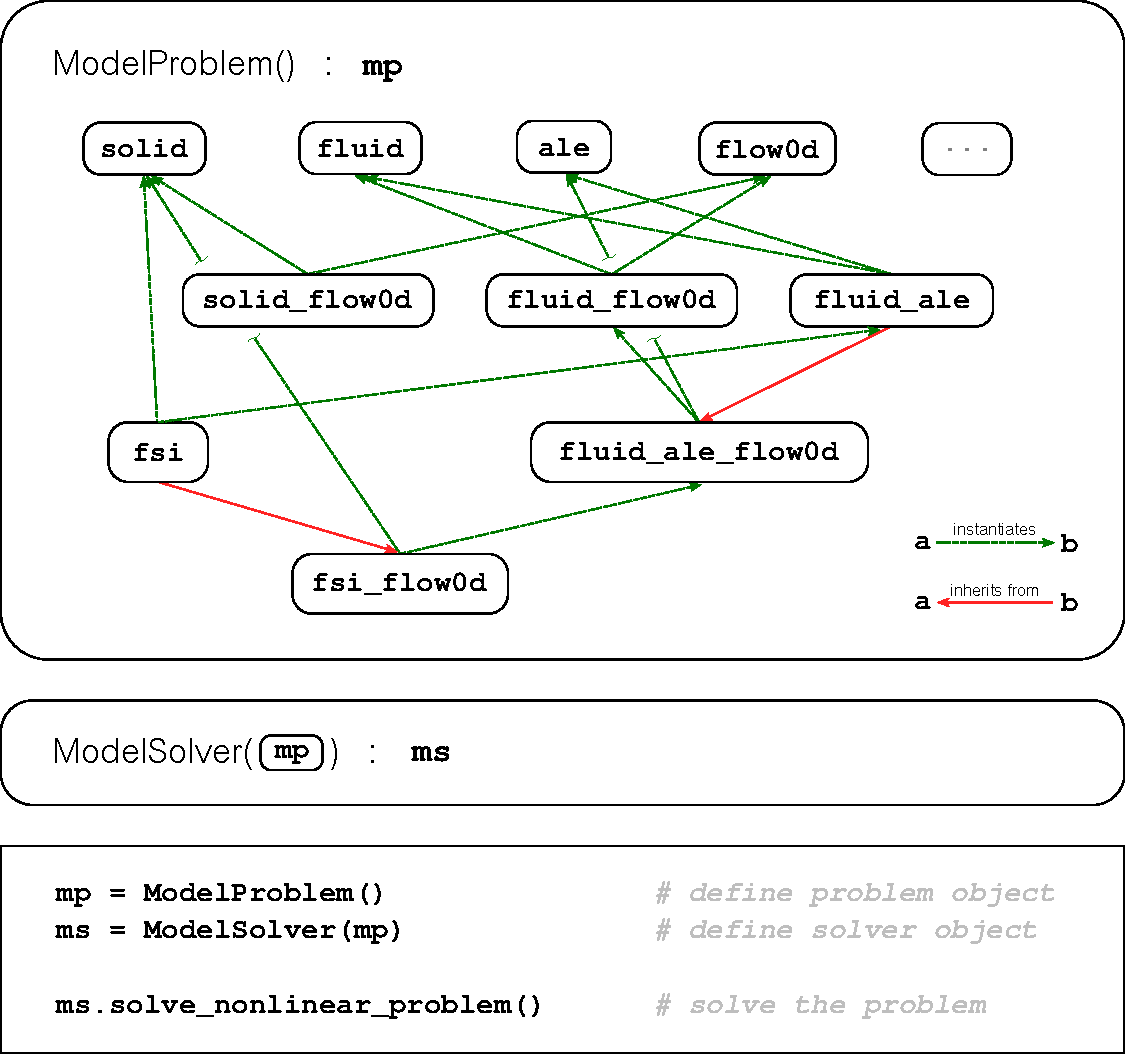
\includegraphics[width=0.8\textwidth]{/home/mh/work/publications/paper_ambit/code_design.pdf}
%\caption{Code design}\label{fig:code_design}
%\end{figure}

\section{Installation}\label{installation}

In order to use Ambit, you need to install FEniCSx (https://github.com/FEniCS/dolfinx\#installation) (latest Ambit-compatible dolfinx development version dates to 19 Aug 2023).\\

Ambit can then be installed using pip, either the current release
\begin{verbatim}
python3 -m pip install ambit-fe
\end{verbatim}

or latest development version:
\begin{verbatim}
python3 -m pip install git+https://github.com/marchirschvogel/ambit.git
\end{verbatim}

Alternatively, you can pull a pre-built Docker image with FEniCSx and Ambit installed:
\begin{verbatim}
docker pull ghcr.io/marchirschvogel/ambit:latest
\end{verbatim}

If a Docker image for development is desired, the following image contains all dependencies needed to install and run Ambit (including the dolfinx mixed branch):
\begin{verbatim}
docker pull ghcr.io/marchirschvogel/ambit:devenv
\end{verbatim}

\section{Ambit input}

Here, a minimal Ambit input file is shown, exemplarily for a single-field problem. The mandatory parameter dictionaries to provide are input parameters (IO), time parameters (TME), solver parameters (SOL), finite element parameters (FEM), and constitutive/material parameters (MAT). For multi-physics problems, each field needs individual time, finite element, and constitutive parameters.

\begin{Verbatim}[breaklines=true]
#!/usr/bin/env python3

# Minimal input file for an elastodynamics problem

import ambit_fe
import numpy as np

def main():

    # Input/output
    IO = {"problem_type"        : "solid",                   # type of physics to solve
          "mesh_domain"         : "/path/mesh_d.xdmf",       # path to domain mesh
          "mesh_boundary"       : "/path/mesh_b.xdmf",       # ath to boundary mesh
          "meshfile_type"       : "HDF5",                    # encoding (HDF5 or ASCII)
          "write_results_every" : 1,                         # step frequency for output
          "output_path"         : "/path/...",               # path to output to
          "results_to_write"    : ["displacement",
                                   "vonmises_cauchystress"], # results to output
          "simname"             : "my_results_name"}         # midfix of output name
    
    # Time discretization  
    TME = {"maxtime"            : 1.0,        # maximum simulation time
           "dt"                 : 0.01,       # time step size
           "timint"             : "genalpha", # time integration: Generalized-alpha
           "rho_inf_genalpha"   : 1.0}        # spectral radius of Gen-alpha scheme
    
    # Solver
    SOL = {"solve_type"         : "direct", # direct linear solver
           "tol_res"            : 1.0e-8,   # residual tolerance
           "tol_inc"            : 1.0e-8}   # increment tolerance
    
    # Finite element discretization
    FEM = {"order_disp"         : 1, # FEM degree for displacement field
           "quad_degree"        : 2} # quadrature scheme degree
    
    # Time curves
    class TC:
        # user defined load curves, to be used in boundary conditions (BC)
        def tc1(self, t):
            load_max = 5.0
            return load_max * np.sin(t)

    # Materials
    MAT = {"MAT1" : {"neohooke_dev" : {"mu" : 10.0},      # isochoric NeoHookean material
                     "ogden_vol"    : {"kappa" : 1.0e3},  # volumetric Ogden material
                     "inertia"      : {"rho0" : 1.0e-6}}} # density

    # Boundary conditions
    BC = {"dirichlet" : [{"id" : [<SURF_IDs>], # list of surfaces for Dirichlet BC
                          "dir" : "all",       # all directions
                          "val" : 0.0}],       # set to zero
          "neumann"   : [{"id" : [<SURF_IDs>], # list of surfaces for Neumann BC
                          "dir" : "xyz_ref",   # in cartesian reference directions
                          "curve" : [1,0,0]}]} # load in x-direction controlled by curve #1 (see time curves)

    # Problem setup
    problem = ambit_fe.ambit_main.Ambit(io_params=IO, time_params=TME, solver_params=SOL, fem_params=FEM, constitutive_params=MAT, boundary_conditions=BC, time_curves=TC)

    # Run: solve the problem
    problem.solve_problem()
    
if __name__ == "__main__":

    main()
\end{Verbatim}

\section{Physics Models}\label{physics-models}

\subsection{Solid mechanics}\label{solid-mechanics}

-- Example: Sec. \ref{demo-solid} and \verb"demos/solid"\\

-- \verb.problem_type : "solid".\\

-- Solid mechanics are formulated in a Total Lagrangian frame

\subsubsection{Strong form}

\textbf{Displacement-based}\\

-- Primary variable: displacement $\bs{u}$
\begin{equation}
\label{equation-solid-strong-form}
\begin{aligned}
\bs{\nabla}_{0} \cdot \bs{P}(\bs{u},\bs{v}(\bs{u})) + \hat{\bs{b}}_{0} &= \rho_{0} \bs{a}(\bs{u}) &&\text{in} \; \mathit{\Omega}_{0} \times [0, T], \\
\bs{u} &= \hat{\bs{u}} &&\text{on} \; \mathit{\Gamma}_{0}^{\mathrm{D}} \times [0, T],\\
\bs{t}_{0} = \bs{P}\bs{n}_{0} &= \hat{\bs{t}}_{0} &&\text{on} \; \mathit{\Gamma}_{0}^{\mathrm{N}} \times [0, T],\\
\bs{u}(\bs{x}_{0},0) &= \hat{\bs{u}}_{0}(\bs{x}_{0}) &&\text{in} \; \mathit{\Omega}_{0},\\
\bs{v}(\bs{x}_{0},0) &= \hat{\bs{v}}_{0}(\bs{x}_{0}) &&\text{in} \; \mathit{\Omega}_{0},
\end{aligned}
\end{equation}

\textbf{Incompressible mechanics}\\

-- Primary variables: displacement $\bs{u}$ and pressure $p$
\begin{equation}
\label{equation-solid-strong-form-inc}
\begin{aligned}
\bs{\nabla}_{0} \cdot \bs{P}(\bs{u},p,\bs{v}(\bs{u})) + \hat{\bs{b}}_{0} &= \rho_{0} \bs{a}(\bs{u}) &&\text{in} \; \mathit{\Omega}_{0} \times [0, T], \\
J(\bs{u})-1 &= 0 &&\text{in} \; \mathit{\Omega}_{0} \times [0, T], \\
\bs{u} &= \hat{\bs{u}} &&\text{on} \; \mathit{\Gamma}_{0}^{\mathrm{D}} \times [0, T],\\
\bs{t}_{0} = \bs{P}\bs{n}_{0} &= \hat{\bs{t}}_{0} &&\text{on} \; \mathit{\Gm}_{0}^{\mathrm{N}} \times [0, T],\\
\bs{u}(\bs{x}_{0},0) &= \hat{\bs{u}}_{0}(\bs{x}_{0}) &&\text{in} \; \mathit{\Om}_{0},\\
\bs{v}(\bs{x}_{0},0) &= \hat{\bs{v}}_{0}(\bs{x}_{0}) &&\text{in} \; \mathit{\Om}_{0},
\end{aligned}
\end{equation}

\subsubsection{Weak form}

\textbf{Displacement-based}\\

-- Primary variable: displacement $\bs{u}$\\

-- Principal of Virtual Work:
\begin{equation}
\label{equation-solid-weak-form}
\begin{aligned}
r(\bs{u};\delta\bs{u}) := \delta \mathcal{W}_{\mathrm{kin}}(\bs{u};\delta\bs{u}) + \delta \mathcal{W}_{\mathrm{int}}(\bs{u};\delta\bs{u}) - \delta \mathcal{W}_{\mathrm{ext}}(\bs{u};\delta\bs{u}) = 0, \quad \forall \; \delta\bs{u}\end{aligned}
\end{equation}
-- Kinetic virtual work:
\begin{equation}
\label{equation-deltaw-kin}
\begin{aligned}
\delta \mathcal{W}_{\mathrm{kin}}(\bs{u};\delta\bs{u}) &= \int\limits_{\Om_{0}} \rho_{0}\,\bs{a}(\bs{u}) \cdot \delta\bs{u} \,\mathrm{d}V
\end{aligned}
\end{equation}
-- Internal virtual work:
\begin{equation}
\label{equation-deltaw-int}
\begin{aligned}
\delta \mathcal{W}_{\mathrm{int}}(\bs{u};\delta\bs{u}) &= \int\limits_{\Om_{0}} \bs{P}(\bs{u},\bs{v}(\bs{u})) : \bs{\nabla}_{0} \delta\bs{u} \,\mathrm{d}V = \int\limits_{\Om_{0}} \bs{S}(\bs{u},\bs{v}(\bs{u})) : \frac{1}{2}\delta\bs{C}(\bs{u}) \,\mathrm{d}V
\end{aligned}
\end{equation}
-- External virtual work:\\
\begin{itemize}
\item conservative Neumann load:
\begin{equation}
\label{equation-deltaw-ext-pk1}
\begin{aligned}
\delta \mathcal{W}_{\mathrm{ext}}(\delta\bs{u}) &= \int\limits_{\Gm_{0}^{\mathrm{N}}} \hat{\bs{t}}_{0}(t) \cdot \delta\bs{u} \,\mathrm{d}A
\end{aligned}
\end{equation}
%-- add to the dict of boundary conditions:\\
%\adjustbox{width=.95\columnwidth}{%
%\verb\"neumann" : [{"id" : [<IDs>], "dir" : "xyz_ref", "curve" : [<#X>,<#Y>,<#Z>]}\
%}%
\item Neumann pressure load in current normal direction:
\begin{equation}
\label{equation-deltaw-ext-cur-p}
\begin{aligned}
\delta \mathcal{W}_{\mathrm{ext}}(\bs{u};\delta\bs{u}) &= -\int\limits_{\Gm_{0}^{\mathrm{N}}} \hat{p}(t)\,J \bs{F}^{-\mathrm{T}}\bs{n}_{0} \cdot \delta\bs{u} \,\mathrm{d}A \end{aligned}
\end{equation}
\item general Neumann load in current direction:
\begin{equation}
\label{equation-deltaw-ext-cur}
\begin{aligned}
\delta \mathcal{W}_{\mathrm{ext}}(\bs{u};\delta\bs{u}) &= \int\limits_{\Gm_0} J\boldsymbol{F}^{-\mathrm{T}}\,\hat{\boldsymbol{t}}_{0}(t) \cdot \delta\boldsymbol{u} \,\mathrm{d}A
\end{aligned}
\end{equation}
\item body force:
\begin{equation}
\label{equation-deltaw-ext-body}
\begin{aligned}
\delta \mathcal{W}_{\mathrm{ext}}(\delta\bs{u}) &= \int\limits_{\Om_{0}} \hat{\bs{b}}_{0}(t) \cdot \delta\bs{u} \,\mathrm{d}V
\end{aligned}
\end{equation}

\item generalized Robin condition:
\begin{equation}
\label{equation-deltaw-ext-robin}
\begin{aligned}
\delta \mathcal{W}_{\mathrm{ext}}(\bs{u};\delta\bs{u}) &= -\int\limits_{\Gm_{0}^{\mathrm{R}}} \left[k\,\bs{u} + c\,\bs{v}(\bs{u})\right] \cdot \delta\bs{u}\,\mathrm{d}A
\end{aligned}
\end{equation}
\item generalized Robin condition in reference surface normal direction:
\begin{equation}
\label{equation-deltaw-ext-robin-n}
\begin{aligned}
\delta \mathcal{W}_{\mathrm{ext}}(\bs{u};\delta\bs{u}) &= -\int\limits_{\Gm_{0}^{\mathrm{R}}} (\bs{n}_0 \otimes \bs{n}_0)\left[k\,\bs{u} + c\,\bs{v}(\bs{u})\right] \cdot \delta\bs{u}\,\mathrm{d}A
\end{aligned}
\end{equation}

\end{itemize}

\textbf{Incompressible mechanics: 2-field displacement and pressure variables}\\

-- Primary variables: displacement $\bs{u}$ and pressure $p$
\begin{equation}
\label{equation-solid-weak-form-inc}
\begin{aligned}
r_u(\bs{u},p;\delta\bs{u}) &:= \delta \mathcal{W}_{\mathrm{kin}}(\bs{u};\delta\bs{u}) + \delta \mathcal{W}_{\mathrm{int}}(\bs{u},p;\delta\bs{u}) - \delta \mathcal{W}_{\mathrm{ext}}(\bs{u};\delta\bs{u}) = 0, \quad \forall \; \delta\bs{u} \\
r_p(\bs{u};\delta p) &:= \delta \mathcal{W}_{\mathrm{pres}}(\bs{u};\delta p) = 0, \quad \forall \; \delta p
\end{aligned}
\end{equation}

-- Kinetic virtual work: (\ref{equation-deltaw-kin})\\
-- Internal virtual work:
\begin{equation}
\label{equation-deltaw-int-inc}
\begin{aligned}
\delta \mathcal{W}_{\mathrm{int}}(\bs{u},p;\delta\bs{u}) &= \int\limits_{\Om_{0}} \bs{P}(\bs{u},p,\bs{v}(\bs{u})) : \bs{\nabla}_{0} \delta\bs{u} \,\mathrm{d}V = \int\limits_{\Om_{0}} \bs{S}(\bs{u},p,\bs{v}(\bs{u})) : \frac{1}{2}\delta\bs{C}(\bs{u}) \,\mathrm{d}V
\end{aligned}
\end{equation}
-- Pressure virtual work:
\begin{equation}
\label{equation-deltaw-p}
\begin{aligned}
\delta \mathcal{W}_{\mathrm{pres}}(\bs{u};\delta p) &= \int\limits_{\Om_{0}} (J(\bs{u}) - 1) \,\delta p \,\mathrm{d}V 
\end{aligned}
\end{equation}


\textbf{Material models}\\
-- hyperelastic material models
\begin{equation}
\begin{aligned}
\bs{S} = 2\frac{\partial\mathit{\Psi}}{\partial \bs{C}}
\end{aligned}
\end{equation}

- MAT \verb."neohooke_dev".\\

\begin{equation}
\begin{aligned}
\mathit{\Psi} &= \frac{\mu}{2}\left(\bar{I}_C - 3\right)
\end{aligned}
\end{equation}


- MAT \verb."holzapfelogden_dev".\\
\begin{equation}
\begin{aligned}
\mathit{\Psi} &= \frac{a_0}{2b_0}\left(e^{b_0(\bar{I}_C - 3)} - 1\right) + \sum\limits_{i\in\{f,s\}}\frac{a_i}{2b_i}\left(e^{b_i(I_{4,i}-1)^2}-1\right) + \frac{a_{fs}}{2b_{fs}}\left(e^{b_{fs}I_{8}^2} - 1\right), \\ & I_{4,f} = \bs{f}_0 \cdot \bs{C}\bs{f}_0, \quad I_{4,s} = \bs{s}_0 \cdot \bs{C}\bs{s}_0, \quad I_8 = \bs{f}_0 \cdot \bs{C}\bs{s}_0
\end{aligned}
\end{equation}

-- viscous material models
\begin{equation}
\begin{aligned}
\bs{S} = 2\frac{\partial\mathit{\Psi}_{\mathrm{v}}}{\partial \dot{\bs{C}}}
\end{aligned}
\end{equation}

\textbf{Time integration}\\

-- time scheme \verb.timint : "static".\\
\begin{equation}
\begin{aligned}
\delta \mathcal{W}_{\mathrm{int}}(\bs{u}_{n+1};\delta\bs{u}) - \delta \mathcal{W}_{\mathrm{ext}}(\bs{u}_{n+1};\delta\bs{u}) = 0, \quad \forall \; \delta\bs{u}\end{aligned}
\end{equation}
-- Generalized-alpha time scheme \verb.timint : "genalpha".
\begin{equation}
\begin{aligned}
\bs{v}_{n+1} &= \frac{\gamma}{\beta\Delta t}(\bs{u}_{n+1}-\bs{u}_{n}) - \frac{\gamma-\beta}{\beta} \bs{v}_{n} - \frac{\gamma-2\beta}{2\beta}\Delta t\,\bs{a}_{n} \\
\bs{a}_{n+1} &= \frac{1}{\beta\Delta t^2}(\bs{u}_{n+1}-\bs{u}_{n}) - \frac{1}{\beta\Delta t} \bs{v}_{n} - \frac{1-2\beta}{2\beta}\bs{a}_{n}
\end{aligned}
\end{equation}
\quad - option \verb.eval_nonlin_terms : "midpoint".:
\begin{equation}
\label{equation-solid-midpoint-genalpha}
\begin{aligned}
\bs{u}_{n+1-\alpha_{\mathrm{f}}} &= (1-\alpha_{\mathrm{f}})\bs{u}_{n+1} + \alpha_{\mathrm{f}} \bs{v}_{n} \\
\bs{v}_{n+1-\alpha_{\mathrm{f}}} &= (1-\alpha_{\mathrm{f}})\bs{v}_{n+1} + \alpha_{\mathrm{f}} \bs{v}_{n} \\
\bs{a}_{n+1-\alpha_{\mathrm{m}}} &= (1-\alpha_{\mathrm{m}})\bs{a}_{n+1} + \alpha_{\mathrm{m}} \bs{a}_{n}
\end{aligned}
\end{equation}
\begin{equation}
\begin{aligned}
\delta \mathcal{W}_{\mathrm{kin}}(\bs{a}_{n+1-\alpha_{m}};\delta\bs{u}) + \delta \mathcal{W}_{\mathrm{int}}(\bs{u}_{n+1-\alpha_{f}};\delta\bs{u}) - \delta \mathcal{W}_{\mathrm{ext}}(\bs{u}_{n+1-\alpha_{f}};\delta\bs{u}) = 0, \quad \forall \; \delta\bs{u}\end{aligned}
\end{equation}
\quad - option \verb.eval_nonlin_terms : "trapezoidal".:
\begin{equation}
\begin{aligned}
&(1-\alpha_{\mathrm{m}})\,\delta \mathcal{W}_{\mathrm{kin}}(\bs{a}_{n+1};\delta\bs{u}) + \alpha_{\mathrm{m}}\,\delta \mathcal{W}_{\mathrm{kin}}(\bs{a}_{n};\delta\bs{u}) + \\
& (1-\alpha_{\mathrm{f}})\,\delta \mathcal{W}_{\mathrm{int}}(\bs{u}_{n+1};\delta\bs{u}) + \alpha_{\mathrm{f}}\,\delta \mathcal{W}_{\mathrm{int}}(\bs{u}_{n};\delta\bs{u}) - \\
& (1-\alpha_{f})\,\delta \mathcal{W}_{\mathrm{ext}}(\bs{u}_{n+1};\delta\bs{u}) - \alpha_{\mathrm{f}}\,\delta \mathcal{W}_{\mathrm{ext}}(\bs{u}_{n};\delta\bs{u}) = 0, \quad \forall \; \delta\bs{u}\end{aligned}
\end{equation}

-- One-Step-theta time scheme \verb.timint : "ost".\\

\begin{equation}
\begin{aligned}
\bs{v}_{n+1} &= \frac{1}{\theta\Delta t}(\bs{u}_{n+1}-\bs{u}_{n}) - \frac{1-\theta}{\theta} \bs{v}_{n} \\
\bs{a}_{n+1} &= \frac{1}{\theta^2\Delta t^2}(\bs{u}_{n+1}-\bs{u}_{n}) - \frac{1}{\theta^2\Delta t} \bs{v}_{n} - \frac{1-\theta}{\theta}\bs{a}_{n}
\end{aligned}
\end{equation}
\quad - option \verb.eval_nonlin_terms : "midpoint".:
\begin{equation}
\label{equation-solid-midpoint-ost}
\begin{aligned}
\bs{u}_{n+\theta} &= \theta \bs{u}_{n+1} + (1-\theta) \bs{u}_{n} \\
\bs{v}_{n+\theta} &= \theta \bs{v}_{n+1} + (1-\theta) \bs{v}_{n} \\
\bs{a}_{n+\theta} &= \theta \bs{a}_{n+1} + (1-\theta) \bs{a}_{n}
\end{aligned}
\end{equation}
\begin{equation}
\begin{aligned}
\delta \mathcal{W}_{\mathrm{kin}}(\bs{a}_{n+\theta};\delta\bs{u}) + \delta \mathcal{W}_{\mathrm{int}}(\bs{u}_{n+\theta};\delta\bs{u}) - \delta \mathcal{W}_{\mathrm{ext}}(\bs{u}_{n+\theta};\delta\bs{u}) = 0, \quad \forall \; \delta\bs{u}\end{aligned}
\end{equation}
\quad - option \verb.eval_nonlin_terms : "trapezoidal".:
\begin{equation}
\begin{aligned}
&\theta\,\delta \mathcal{W}_{\mathrm{kin}}(\bs{a}_{n+1};\delta\bs{u}) + (1-\theta)\,\delta \mathcal{W}_{\mathrm{kin}}(\bs{a}_{n};\delta\bs{u}) + \\
& \theta\,\delta \mathcal{W}_{\mathrm{int}}(\bs{u}_{n+1};\delta\bs{u}) + (1-\theta)\,\delta \mathcal{W}_{\mathrm{int}}(\bs{u}_{n};\delta\bs{u}) - \\
& \theta\,\delta \mathcal{W}_{\mathrm{ext}}(\bs{u}_{n+1};\delta\bs{u}) - (1-\theta)\,\delta \mathcal{W}_{\mathrm{ext}}(\bs{u}_{n};\delta\bs{u}) = 0, \quad \forall \; \delta\bs{u}
\end{aligned}
\end{equation}

Note the equivalence of \verb."midpoint". and \verb."trapezoidal". for all linear terms, e.g. $\delta \mathcal{W}_{\mathrm{kin}}$, or for no or only linear dependence of $\delta \mathcal{W}_{\mathrm{ext}}$ on the solution.\\

Note that, for incompressible mechanics, the pressure kinematic constraint is always evaluated at $t_{n+1}$:
\begin{equation}
\begin{aligned}
\delta \mathcal{W}_{\mathrm{pres}}(\bs{u}_{n+1};\delta p) = 0, \quad \forall \; \delta p,
\end{aligned}
\end{equation}
and the pressure in $\delta \mathcal{W}_{\mathrm{int}}$ is set according to (\ref{equation-solid-midpoint-genalpha}) or (\ref{equation-solid-midpoint-ost}), respectively.

\textbf{Spatial discretization and solution}\\

-- Discrete nonlinear system to solve in each time step $n$ (displacement-based):
\begin{equation}
\label{equation-nonlin-sys-solid}
\begin{aligned}
\left.\ROP_{u}(\bs{\mathsf{u}})\right|_{n+1} = \bs{\mathsf{0}}
\end{aligned}
\end{equation}

-- Discrete linear system to solve in each Newton iteration $k$ (displacement-based):
\begin{equation}
\label{equation-lin-sys-solid}
\begin{aligned}
\left. \bs{\mathsf{K}}_{uu} \right|_{n+1}^{k} \Delta\bs{\mathsf{u}}_{n+1}^{k+1}=-\left. \ROP_{u} \right|_{n+1}^{k}
\end{aligned}
\end{equation}

-- Discrete nonlinear system to solve in each time step $n$ (incompressible):
\begin{equation}
\label{equation-nonlin-sys-solid-inc}
\begin{aligned}
\ROP_{n+1} = \begin{bmatrix} \ROP_{u}(\bs{\mathsf{u}},\bs{\mathsf{p}}) \\ \ROP_{p}(\bs{\mathsf{u}}) \end{bmatrix}_{n+1} = \bs{\mathsf{0}}
\end{aligned}
\end{equation}

-- Discrete linear system to solve in each Newton iteration $k$ (incompressible):
\begin{equation}
\label{equation-lin-sys-solid-inc}
\begin{aligned}
\begin{bmatrix} \bs{\mathsf{K}}_{uu} & \bs{\mathsf{K}}_{up} \\ \\ \bs{\mathsf{K}}_{pu} & \zerom \end{bmatrix}_{n+1}^{k}\begin{bmatrix} \Delta\bs{\mathsf{u}} \\ \\ \Delta\bs{\mathsf{p}} \end{bmatrix}_{n+1}^{k+1}=-\begin{bmatrix} \ROP_{u} \\ \\ \ROP_{p} \end{bmatrix}_{n+1}^{k}
\end{aligned}
\end{equation}




\subsection{Fluid mechanics}\label{fluid-mechanics}

\subsubsection{Eulerian reference frame}\label{eulerian-reference-frame}

-- Example: Sec. \ref{demo-fluid} and \verb"demos/fluid"\\

-- Problem type: \verb.fluid.\\

-- Incompressible Navier-Stokes equations in Eulerian reference frame\\

\textbf{Strong Form}\\

-- Primary variables: velocity $\bs{v}$ and pressure $p$
\begin{equation}
\label{equation-fluid-strong-form}
\begin{aligned}
\bs{\nabla} \cdot \bs{\sigma}(\bs{v},p) + \hat{\bs{b}} &= \rho\left(\frac{\partial\bs{v}}{\partial t} + (\bs{\nabla}\bs{v})\,\bs{v}\right) &&\text{in} \; \mathit{\Om}_t \times [0, T], \\
\bs{\nabla}\cdot \bs{v} &= 0 &&\text{in} \; \mathit{\Om}_t \times [0, T],\\
\bs{v} &= \hat{\bs{v}} &&\text{on} \; \mathit{\Gm}_t^{\mathrm{D}} \times [0, T],\\
\bs{t} = \bs{\sigma}\bs{n} &= \hat{\bs{t}} &&\text{on} \; \mathit{\Gm}_t^{\mathrm{N}} \times [0, T],\\
\bs{v}(\bs{x},0) &= \hat{\bs{v}}_{0}(\bs{x}) &&\text{in} \; \mathit{\Om}_t,
\end{aligned}
\end{equation}

with a Newtonian fluid constitutive law
\begin{align}
\bs{\sigma} = -p \bs{I} + 2 \mu\,\bs{\gamma} = -p \bs{I} + \mu \left(\bs{\nabla} \bs{v} + (\bs{\nabla} \bs{v})^{\mathrm{T}}\right)
\end{align}

\textbf{Weak Form}\\

-- Primary variables: velocity $\bs{v}$ and pressure $p$\\

-- Principle of Virtual Power
\begin{equation}
\label{equation-fluid-weak-form}
\begin{aligned}
r_v(\bs{v},p;\delta\bs{v}) &:= \delta \mathcal{P}_{\mathrm{kin}}(\bs{v};\delta\bs{v}) + \delta \mathcal{P}_{\mathrm{int}}(\bs{v},p;\delta\bs{v}) - \delta \mathcal{P}_{\mathrm{ext}}(\bs{v};\delta\bs{v}) = 0, \quad \forall \; \delta\bs{v} \\
r_p(\bs{v};\delta p) &:= \delta \mathcal{P}_{\mathrm{pres}}(\bs{v};\delta p), \quad \forall \; \delta p
\end{aligned}
\end{equation}

-- Kinetic virtual power:
\begin{equation}
\label{equation-deltap-kin}
\begin{aligned}
\delta \mathcal{P}_{\mathrm{kin}}(\bs{v};\delta\bs{v}) = \int\limits_{\Om_t} \rho\left(\frac{\partial\bs{v}}{\partial t} + (\bs{\nabla}\bs{v})\,\bs{v}\right) \cdot \delta\bs{v} \,\mathrm{d}v
\end{aligned}
\end{equation}
-- Internal virtual power:
\begin{equation}
\label{equation-deltap-int}
\begin{aligned}
\delta \mathcal{P}_{\mathrm{int}}(\bs{v},p;\delta\bs{v}) = 
\int\limits_{\Om_t} \bs{\sigma}(\bs{v},p) : \bs{\nabla} \delta\bs{v} \,\mathrm{d}v 
\end{aligned}
\end{equation}

-- Pressure virtual power:
\begin{equation}
\label{equation-deltap-p}
\begin{aligned}
\delta \mathcal{P}_{\mathrm{pres}}(\bs{v};\delta p) = 
\int\limits_{\Om_t} (\bs{\nabla}\cdot\bs{v})\,\delta p\,\mathrm{d}v
\end{aligned}
\end{equation}

-- External virtual power:\\
\begin{itemize}
\item conservative Neumann load:
\begin{equation}
\label{equation-deltap-ext-cur}
\begin{aligned}
\delta \mathcal{P}_{\mathrm{ext}}(\delta\bs{v}) &= \int\limits_{\Gm_t^{\mathrm{N}}} \hat{\bs{t}}(t) \cdot \delta\bs{v} \,\mathrm{d}a
\end{aligned}
\end{equation}
\item pressure Neumann load:
\begin{equation}
\label{equation-deltap-ext-cur-p}
\begin{aligned}
\delta \mathcal{P}_{\mathrm{ext}}(\delta\bs{v}) &= -\int\limits_{\Gm_t^{\mathrm{N}}} \hat{p}(t)\,\bs{n} \cdot \delta\bs{v} \,\mathrm{d}a
\end{aligned}
\end{equation}
\item body force:
\begin{equation}
\label{equation-deltap-ext-body}
\begin{aligned}
\delta \mathcal{P}_{\mathrm{ext}}(\delta\bs{v}) &= \int\limits_{\Om_t} \hat{\bs{b}}(t) \cdot \delta\bs{v} \,\mathrm{d}V
\end{aligned}
\end{equation}
\end{itemize}

\textbf{Stabilization}\\

Streamline-upwind Petrov-Galerkin/pressure-stabilizing Petrov-Galerkin (SUPG/PSPG) methods are implemented, either using the full or a reduced scheme\\

-- to the fluid FEM params, add the dict entry:

\begin{Verbatim}[breaklines=true]
"stabilization" : {"scheme" : <SCHEME>, "vscale" : 1e3, "dscales" : [<d1>,<d2>,<d3>],
                   "symmetric" : False}
\end{Verbatim}

Full scheme according to \cite{tezduyar2000}: \verb."supg_pspg".:\\
-- Velocity residual operator in (\ref{equation-fluid-weak-form}) is augmented by the following terms:
\begin{equation}
\begin{aligned}
r_v \leftarrow r_v &+ \frac{1}{\rho}\int\limits_{\Om_t} \tau_{\mathrm{SUPG}}\,(\bs{\nabla}\delta\bs{v})\,\bs{v} \cdot \left[\rho\left(\frac{\partial \bs{v}}{\partial t} + (\bs{\nabla}\bs{v})\,\bs{v}\right) - \bs{\nabla} \cdot \bs{\sigma}(\bs{v},p)\right]\,\mathrm{d}v \\
& + \int\limits_{\Om_t} \tau_{\mathrm{LSIC}}\,\rho\,(\bs{\nabla}\cdot\delta\bs{v})(\bs{\nabla}\cdot\bs{v})\,\mathrm{d}v
\end{aligned}
\end{equation}
-- Pressure residual operator in (\ref{equation-fluid-weak-form}) is augmented by the following terms:
\begin{equation}
\begin{aligned}
r_p \leftarrow r_p &+ \frac{1}{\rho}\int\limits_{\Om_t} \tau_{\mathrm{PSPG}}\,(\bs{\nabla}\delta p) \cdot \left[\rho\left(\frac{\partial \bs{v}}{\partial t} + (\bs{\nabla}\bs{v})\,\bs{v}\right) - \bs{\nabla} \cdot \bs{\sigma}(\bs{v},p)\right]\,\mathrm{d}v 
\end{aligned}
\end{equation}


Reduced scheme (optimized for first-order): \verb."supg_pspg2".:

-- Velocity residual operator in (\ref{equation-fluid-weak-form}) is augmented by the following terms:
\begin{equation}
\begin{aligned}
r_v \leftarrow r_v &+ \int\limits_{\Om_t} d_1\,((\bs{\nabla}\bs{v})\,\bs{v}) \cdot (\bs{\nabla}\delta\bs{v})\,\bs{v}\,\mathrm{d}v \\
& + \int\limits_{\Om_t} d_2\,(\bs{\nabla}\cdot\bs{v}) (\bs{\nabla}\cdot\delta\bs{v})\,\mathrm{d}v\\
&+ \int\limits_{\Om_t} d_3\,(\bs{\nabla}p) \cdot (\bs{\nabla}\delta\bs{v})\,\bs{v}\,\mathrm{d}v 
\end{aligned}
\end{equation}
-- Pressure residual operator in (\ref{equation-fluid-weak-form}) is augmented by the following terms:
\begin{equation}
\begin{aligned}
r_p \leftarrow r_p &+ \frac{1}{\rho}\int\limits_{\Om_t} d_1\,((\bs{\nabla}\bs{v})\,\bs{v}) \cdot (\bs{\nabla}\delta p)\,\mathrm{d}v \\
&+ \frac{1}{\rho}\int\limits_{\Om_t} d_3\,(\bs{\nabla}p) \cdot (\bs{\nabla}\delta p)\,\mathrm{d}v 
\end{aligned}
\end{equation}

-- Discrete nonlinear system to solve in each time step $n$:
\begin{equation}
\label{equation-nonlin-sys-fluid}
\begin{aligned}
\ROP_{n+1} = \begin{bmatrix} \ROP_{v}(\bs{\mathsf{v}},\bs{\mathsf{p}}) \\ \ROP_{p}(\bs{\mathsf{p}},\bs{\mathsf{v}}) \end{bmatrix}_{n+1} = \bs{\mathsf{0}}
\end{aligned}
\end{equation}

-- Discrete linear system to solve in each Newton iteration $k$:
\begin{equation}
\label{equation-lin-sys-fluid}
\begin{aligned}
\begin{bmatrix} \bs{\mathsf{K}}_{vv} & \bs{\mathsf{K}}_{vp} \\ \\ \bs{\mathsf{K}}_{pv} & \bs{\mathsf{K}}_{pp} \end{bmatrix}_{n+1}^{k}\begin{bmatrix} \Delta\bs{\mathsf{v}} \\ \\ \Delta\bs{\mathsf{p}} \end{bmatrix}_{n+1}^{k+1}=-\begin{bmatrix} \ROP_{v} \\ \\ \ROP_{p} \end{bmatrix}_{n+1}^{k}
\end{aligned}
\end{equation}
-- Note that $\bs{\mathsf{K}}_{pp}$ is zero for Taylor-Hood elements (without stabilization)

\subsubsection{ALE reference frame}\label{ale-reference-frame}

-- Problem type: \verb.fluid_ale.\\

-- Incompressible Navier-Stokes equations in Arbitrary Lagrangian Eulerian (ALE) reference frame\\

-- ALE domain problem deformation governed by linear-elastic, nonlinear hyperelastic solid, or a diffusion problem, displacement field $\bs{d}$\\

-- Fluid mechanics formulated with respect to the reference frame, using ALE deformation gradient $\widetilde{\bs{F}}(\bs{d}) = \bs{I} + \bs{\nabla}_0\bs{d}$ and its determinant, $\widetilde{J}(\bs{d})=\det \widetilde{\bs{F}}(\bs{d})$\\

\textbf{ALE problem}\\

-- Primary variable: domain displacement $\bs{d}$\\

-- Strong form:
\begin{equation}
\label{equation-ale-strong-form}
\begin{aligned}
\bs{\nabla}_{0} \cdot \bs{\sigma}^{\mathrm{G}}(\bs{d}) &= \bs{0} &&\text{in} \; \mathit{\Om}_0, \\
\bs{d} &= \hat{\bs{d}} &&\text{on} \; \mathit{\Gm}_0^{\mathrm{D}},
\end{aligned}
\end{equation}
-- ALE material \verb.linelast.:
\begin{equation}
\begin{aligned}
\bs{\sigma}^{\mathrm{G}}(\bs{d}) = 2\mu \,\bs{\varepsilon} + \lambda \,\mathrm{tr}\bs{\varepsilon}\,\bs{I}, \qquad \text{with}\quad \bs{\varepsilon} = \frac{1}{2}\left(\bs{\nabla}_0\bs{d} + (\bs{\nabla}_0\bs{d})^{\mathrm{T}}\right)
\end{aligned}
\end{equation}
-- ALE material \verb.diffusion.:
\begin{equation}
\begin{aligned}
\bs{\sigma}^{\mathrm{G}}(\bs{d}) = D \,\bs{\nabla}_0\bs{d}
\end{aligned}
\end{equation}
-- ALE material \verb.neohooke. (fully nonlinear model):
\begin{equation}
\begin{aligned}
\bs{\sigma}^{\mathrm{G}}(\bs{d}) = \frac{\partial \mathit{\Psi}}{\partial \widetilde{\bs{F}}}, \qquad \text{with}\quad \mathit{\Psi} = \frac{\mu}{2}\left(\mathrm{tr}(\widetilde{\bs{F}}^{\mathrm{T}}\widetilde{\bs{F}}) - 3\right) + \frac{\mu}{2\beta} \left(\widetilde{J}^{-2\beta} - 1\right)
\end{aligned}
\end{equation}

-- weak form:
\begin{equation}
\label{equation-ale-weak-form}
\begin{aligned}
r_{d}(\bs{d};\delta\bs{d}) := \int\limits_{\Om_0}\bs{\sigma}^{\mathrm{G}}(\bs{d}) : \bs{\nabla}_{0}\delta\bs{d}\,\mathrm{d}V = 0, \quad \forall \; \delta\bs{d}
\end{aligned}
\end{equation}


\textbf{Strong form (ALE)}\\

-- Primary variables: velocity $\bs{v}$, pressure $p$, and domain displacement $\bs{d}$
\begin{equation}
\label{equation-fluid-ale-strong-form}
\begin{aligned}
\bs{\nabla}_{0} \bs{\sigma}(\bs{v},\bs{d},p) : \widetilde{\bs{F}}^{-\mathrm{T}} + \hat{\bs{b}} &= \rho\left(\frac{\partial\bs{v}}{\partial t} + (\bs{\nabla}_0\bs{v}\,\widetilde{\bs{F}}^{-1})\,(\bs{v}-\bs{w})\right) &&\text{in} \; \mathit{\Om}_0 \times [0, T],\\
\bs{\nabla}_{0}\bs{v} : \widetilde{\bs{F}}^{-\mathrm{T}} &= 0 &&\text{in} \; \mathit{\Om}_0 \times [0, T],\\
\bs{v} &= \hat{\bs{v}} &&\text{on} \; \mathit{\Gm}_0^{\mathrm{D}} \times [0, T], \\
\bs{t} = \bs{\sigma}\bs{n} &= \hat{\bs{t}} &&\text{on} \; \mathit{\Gm}_0^{\mathrm{N}} \times [0, T], \\
\bs{v}(\bs{x},0) &= \hat{\bs{v}}_{0}(\bs{x}) &&\text{in} \; \mathit{\Om}_0,
\end{aligned}
\end{equation}

with a Newtonian fluid constitutive law
\begin{align}
\bs{\sigma} = -p \bs{I} + 2 \mu \bs{\gamma} = -p \bs{I} + \mu \left(\bs{\nabla}_0 \bs{v}\,\widetilde{\bs{F}}^{-1} + \widetilde{\bs{F}}^{-\mathrm{T}}(\bs{\nabla}_0 \bs{v})^{\mathrm{T}}\right)
\end{align}

\textbf{Weak form (ALE)}\\

-- Primary variables: velocity $\bs{v}$, pressure $p$, and domain displacement $\bs{d}$\\

-- Principle of Virtual Power
\begin{equation}
\label{equation-fluid-ale-weak-form}
\begin{aligned}
r_v(\bs{v},p,\bs{d};\delta\bs{v}) &:= \delta \mathcal{P}_{\mathrm{kin}}(\bs{v},\bs{d};\delta\bs{v}) + \delta \mathcal{P}_{\mathrm{int}}(\bs{v},p,\bs{d};\delta\bs{v}) - \delta \mathcal{P}_{\mathrm{ext}}(\bs{v},\bs{d};\delta\bs{v}) = 0, \quad \forall \; \delta\bs{v} \\
r_p(\bs{v},\bs{d};\delta p) &:= \delta \mathcal{P}_{\mathrm{pres}}(\bs{v},\bs{d};\delta p), \quad \forall \; \delta p
\end{aligned}
\end{equation}

-- Kinetic virtual power:
\begin{equation}
\begin{aligned}
\delta \mathcal{P}_{\mathrm{kin}}(\bs{v},\bs{d};\delta\bs{v}) = \int\limits_{\Om_0} \widetilde{J} \rho\left(\frac{\partial\bs{v}}{\partial t} + (\bs{\nabla}_{0}\bs{v}\,\widetilde{\bs{F}}^{-1})\,(\bs{v}-\bs{w})\right) \cdot \delta\bs{v} \,\mathrm{d}V
\end{aligned}
\end{equation}
-- Internal virtual power:
\begin{equation}
\begin{aligned}
\delta \mathcal{P}_{\mathrm{int}}(\bs{v},p,\bs{d};\delta\bs{v}) = 
\int\limits_{\Om_0} \widetilde{J}\bs{\sigma}(\bs{v},p,\bs{d}) : \bs{\nabla}_{0} \delta\bs{v}\,\widetilde{\bs{F}}^{-1} \,\mathrm{d}V
\end{aligned}
\end{equation}

-- Pressure virtual power:
\begin{equation}
\begin{aligned}
\delta \mathcal{P}_{\mathrm{pres}}(\bs{v},\bs{d};\delta p) = 
\int\limits_{\Om_0} \widetilde{J}\,\bs{\nabla}_{0}\bs{v} : \widetilde{\bs{F}}^{-\mathrm{T}}\delta p\,\mathrm{d}V
\end{aligned}
\end{equation}

-- External virtual power:\\
\begin{itemize}
\item conservative Neumann load:
\begin{equation}
\begin{aligned}
\delta \mathcal{P}_{\mathrm{ext}}(\delta\bs{v}) &= \int\limits_{\Gm_0^{\mathrm{N}}} \hat{\bs{t}}(t) \cdot \delta\bs{v} \,\mathrm{d}A
\end{aligned}
\end{equation}
\item pressure Neumann load:
\begin{equation}
\begin{aligned}
\delta \mathcal{P}_{\mathrm{ext}}(\bs{d};\delta\bs{v}) &= -\int\limits_{\Gm_0^{\mathrm{N}}} \hat{p}(t)\,\widetilde{J}\widetilde{\bs{F}}^{-\mathrm{T}}\bs{n}_{0} \cdot \delta\bs{v} \,\mathrm{d}A 
\end{aligned}
\end{equation}
\item body force:
\begin{equation}
\begin{aligned}
\delta \mathcal{P}_{\mathrm{ext}}(\bs{d};\delta\bs{v}) &= \int\limits_{\Om_0} \widetilde{J}\,\hat{\bs{b}}(t) \cdot \delta\bs{v} \,\mathrm{d}V
\end{aligned}
\end{equation}
\end{itemize}

\textbf{Stabilization (ALE)}\\

\verb."supg_pspg".:\\
-- Velocity residual operator in (\ref{equation-fluid-ale-weak-form}) is augmented by the following terms:
\begin{equation}
\begin{aligned}
r_v \leftarrow r_v &+ \frac{1}{\rho}\int\limits_{\Om_0}\widetilde{J}\, \tau_{\mathrm{SUPG}}\,(\bs{\nabla}_0\delta\bs{v}\,\widetilde{\bs{F}}^{-1})\,\bs{v}\;\cdot \\
& \qquad\quad \cdot\left[\rho\left(\frac{\partial \bs{v}}{\partial t} + (\bs{\nabla}_0\bs{v}\,\widetilde{\bs{F}}^{-1})\,(\bs{v}-\bs{w})\right) - \bs{\nabla}_{0} \bs{\sigma}(\bs{v},\bs{d},p) : \widetilde{\bs{F}}^{-\mathrm{T}}\right]\,\mathrm{d}V \\
& + \int\limits_{\Om_0}\widetilde{J}\, \tau_{\mathrm{LSIC}}\,\rho\,(\bs{\nabla}_{0}\delta\bs{v} : \widetilde{\bs{F}}^{-\mathrm{T}})(\bs{\nabla}_{0}\bs{v} : \widetilde{\bs{F}}^{-\mathrm{T}})\,\mathrm{d}V
\end{aligned}
\end{equation}
-- Pressure residual operator in (\ref{equation-fluid-ale-weak-form}) is augmented by the following terms:
\begin{equation}
\begin{aligned}
r_p \leftarrow r_p &+ \frac{1}{\rho}\int\limits_{\Om_0}\widetilde{J}\, \tau_{\mathrm{PSPG}}\,(\widetilde{\bs{F}}^{-\mathrm{T}}\bs{\nabla}_{0}\delta p) \;\cdot \\
& \qquad\quad \cdot \left[\rho\left(\frac{\partial \bs{v}}{\partial t} + (\bs{\nabla}_0\bs{v}\,\widetilde{\bs{F}}^{-1})\,(\bs{v}-\bs{w})\right) - \bs{\nabla}_{0} \bs{\sigma}(\bs{v},\bs{d},p) : \widetilde{\bs{F}}^{-\mathrm{T}}\right]\,\mathrm{d}V
\end{aligned}
\end{equation}

\verb."supg_pspg2".:\\
-- Velocity residual operator in (\ref{equation-fluid-ale-weak-form}) is augmented by the following terms:
\begin{equation}
\begin{aligned}
r_v \leftarrow r_v &+ \int\limits_{\Om_0} \widetilde{J}\,d_1\,((\bs{\nabla}_{0}\bs{v}\,\widetilde{\bs{F}}^{-1})\,(\bs{v}-\bs{w})) \cdot (\bs{\nabla}_{0}\delta\bs{v}\,\widetilde{\bs{F}}^{-1})\,\bs{v}\,\mathrm{d}V \\
& + \int\limits_{\Om_0} \widetilde{J}\,d_2\,(\bs{\nabla}_{0}\bs{v} : \widetilde{\bs{F}}^{-\mathrm{T}}) (\bs{\nabla}_{0}\delta\bs{v} : \widetilde{\bs{F}}^{-\mathrm{T}})\,\mathrm{d}V\\
&+ \int\limits_{\Om_0} \widetilde{J}\,d_3\,(\widetilde{\bs{F}}^{-\mathrm{T}}\bs{\nabla}_{0}p) \cdot (\bs{\nabla}_{0}\delta\bs{v}\,\widetilde{\bs{F}}^{-1})\,\bs{v}\,\mathrm{d}V
\end{aligned}
\end{equation}
-- Pressure residual operator in (\ref{equation-fluid-ale-weak-form}) is augmented by the following terms:
\begin{equation}
\begin{aligned}
r_p \leftarrow r_p &+ \frac{1}{\rho}\int\limits_{\Om_0} \widetilde{J}\,d_1\,((\bs{\nabla}_{0}\bs{v}\,\widetilde{\bs{F}}^{-1})\,(\bs{v}-\bs{w})) \cdot (\widetilde{\bs{F}}^{-\mathrm{T}}\bs{\nabla}_{0}\delta p)\,\mathrm{d}V \\
&+ \frac{1}{\rho}\int\limits_{\Om_0} \widetilde{J}\,d_3\,(\widetilde{\bs{F}}^{-\mathrm{T}}\bs{\nabla}_{0}p) \cdot (\widetilde{\bs{F}}^{-\mathrm{T}}\bs{\nabla}_{0}\delta p)\,\mathrm{d}V
\end{aligned}
\end{equation}

-- Discrete nonlinear system to solve in each time step $n$:
\begin{equation}
\label{equation-nonlin-sys-fluid-ale}
\begin{aligned}
\ROP_{n+1} = \begin{bmatrix} \ROP_{v}(\bs{\mathsf{v}},\bs{\mathsf{p}},\bs{\mathsf{d}}) \\ \ROP_{p}(\bs{\mathsf{p}},\bs{\mathsf{v}},\bs{\mathsf{d}}) \\ \ROP_{d}(\bs{\mathsf{d}}) \end{bmatrix}_{n+1} = \bs{\mathsf{0}}
\end{aligned}
\end{equation}

-- Discrete linear system to solve in each Newton iteration $k$:
\begin{equation}
\label{equation-lin-sys-fluid-ale}
\begin{aligned}
\begin{bmatrix} \bs{\mathsf{K}}_{vv} & \bs{\mathsf{K}}_{vp} & \bs{\mathsf{K}}_{vd} \\ \\ \bs{\mathsf{K}}_{pv} & \bs{\mathsf{K}}_{pp} & \bs{\mathsf{K}}_{pd} \\ \\ \bs{\mathsf{K}}_{dv}  & \zerom & \bs{\mathsf{K}}_{dd} \end{bmatrix}_{n+1}^{k}\begin{bmatrix} \Delta\bs{\mathsf{v}} \\ \\ \Delta\bs{\mathsf{p}} \\ \\ \Delta\bs{\mathsf{d}} \end{bmatrix}_{n+1}^{k+1}=-\begin{bmatrix} \ROP_{v} \\ \\ \ROP_{p} \\ \\ \ROP_{d} \end{bmatrix}_{n+1}^{k} 
\end{aligned}
\end{equation}
-- note that $\bs{\mathsf{K}}_{pp}$ is zero for Taylor-Hood elements (without stabilization)


\subsection{0D flow: Lumped parameter models}\label{d-flow-lumped-parameter-models}

-- Example: Sec. \ref{demo-0d-flow} and \verb"demos/flow0d"\\

-- Problem type: \verb"flow0d"\\

-- 0D model concentrated elements are resistances ($R$), impedances ($Z$, technically are resistances), compliances ($C$), inertances ($L$ or $I$), and elastances ($E$)\\

-- 0D variables are pressures ($p$), fluxes ($q$ or $Q$), or volumes ($V$)

\subsubsection{2-element Windkessel}

-- Model type : \verb"2elwindkessel"\\

\subsubsection{4-element Windkessel (inertance parallel to impedance)}

-- Model type : \verb"4elwindkesselLpZ"\\

\subsubsection{4-element Windkessel (inertance serial to impedance)}

-- Model type : \verb"4elwindkesselLsZ"\\

\subsubsection{In-outflow CRL link}

-- Model type : \verb"CRLinoutlink"\\

\subsubsection{Systemic and pulmonary circulation}

-- Model type : \verb"syspul"\\

-- Allows to link in a coronary flow model

\begin{equation}
\label{equation-syspul-1}
\begin{aligned}
&\text{left heart and systemic circulation} && \nonumber\\
&-Q_{\mathrm{at}}^{\ell} = \sum\limits_{i=1}^{n_{\mathrm{ven}}^{\mathrm{pul}}}q_{\mathrm{ven},i}^{\mathrm{pul}} - q_{\mathrm{v,in}}^{\ell} && \text{left atrium flow balance}\\
&q_{\mathrm{v,in}}^{\ell} = q_{\mathrm{mv}}(p_{\mathrm{at}}^{\ell}-p_{\mathrm{v}}^{\ell}) && \text{mitral valve momentum}\\
&-Q_{\mathrm{v}}^{\ell} = q_{\mathrm{v,in}}^{\ell} - q_{\mathrm{v,out}}^{\ell} && \text{left ventricle flow balance}\\
&q_{\mathrm{v,out}}^{\ell} = q_{\mathrm{av}}(p_{\mathrm{v}}^{\ell}-p_{\mathrm{ar}}^{\mathrm{sys}}) && \text{aortic valve momentum}\\
&-Q_{\mathrm{aort}}^{\mathrm{sys}} = q_{\mathrm{v,out}}^{\ell} - q_{\mathrm{ar,p}}^{\mathrm{sys}} - \mathbb{I}^{\mathrm{cor}}\sum\limits_{i=1}^{2}q_{\mathrm{ar,cor,in},i}^{\mathrm{sys}} && \text{aortic root flow balance}\\
&I_{\mathrm{ar}}^{\mathrm{sys}} \frac{\mathrm{d}q_{\mathrm{ar,p}}^{\mathrm{sys}}}{\mathrm{d}t} + Z_{\mathrm{ar}}^{\mathrm{sys}}\,q_{\mathrm{ar,p}}^{\mathrm{sys}}=p_{\mathrm{ar}}^{\mathrm{sys}}-p_{\mathrm{ar,d}}^{\mathrm{sys}} && \text{aortic root inertia}\nonumber\\
&C_{\mathrm{ar}}^{\mathrm{sys}} \frac{\mathrm{d}p_{\mathrm{ar,d}}^{\mathrm{sys}}}{\mathrm{d}t} = q_{\mathrm{ar,p}}^{\mathrm{sys}} - q_{\mathrm{ar}}^{\mathrm{sys}} && \text{systemic arterial flow balance}\\
&L_{\mathrm{ar}}^{\mathrm{sys}} \frac{\mathrm{d}q_{\mathrm{ar}}^{\mathrm{sys}}}{\mathrm{d}t} + R_{\mathrm{ar}}^{\mathrm{sys}}\,q_{\mathrm{ar}}^{\mathrm{sys}}=p_{\mathrm{ar,d}}^{\mathrm{sys}}-p_{\mathrm{ven}}^{\mathrm{sys}} && \text{systemic arterial momentum}\\
&C_{\mathrm{ven}}^{\mathrm{sys}} \frac{\mathrm{d}p_{\mathrm{ven}}^{\mathrm{sys}}}{\mathrm{d}t} = q_{\mathrm{ar}}^{\mathrm{sys}}-\sum\limits_{i=1}^{n_{\mathrm{ven}}^{\mathrm{sys}}}q_{\mathrm{ven},i}^{\mathrm{sys}}\ && \text{systemic venous flow balance}\\
&L_{\mathrm{ven},i}^{\mathrm{sys}} \frac{\mathrm{d}q_{\mathrm{ven},i}^{\mathrm{sys}}}{\mathrm{d}t} + R_{\mathrm{ven},i}^{\mathrm{sys}}\, q_{\mathrm{ven},i}^{\mathrm{sys}} = p_{\mathrm{ven}}^{\mathrm{sys}} - p_{\mathrm{at},i}^{r} && \text{systemic venous momentum}\nonumber\\
&\qquad\qquad i \in \{1,...,n_{\mathrm{ven}}^{\mathrm{sys}}\} && 
\end{aligned}
\end{equation}
\begin{equation}
\label{equation-syspul-2}
\begin{aligned}
&\text{right heart and pulmonary circulation} && \\
&-Q_{\mathrm{at}}^{r} = \sum\limits_{i=1}^{n_{\mathrm{ven}}^{\mathrm{sys}}}q_{\mathrm{ven},i}^{\mathrm{sys}} - \mathbb{I}^{\mathrm{cor}} q_{\mathrm{ven,cor,out}}^{\mathrm{sys}} - q_{\mathrm{v,in}}^{r} && \text{right atrium flow balance}\\
&q_{\mathrm{v,in}}^{r} = q_{\mathrm{tv}}(p_{\mathrm{at}}^{r}-p_{\mathrm{v}}^{r}) && \text{tricuspid valve momentum}\\
&-Q_{\mathrm{v}}^{r} = q_{\mathrm{v,in}}^{r} - q_{\mathrm{v,out}}^{r} && \text{right ventricle flow balance}\\
&q_{\mathrm{v,out}}^{r} = q_{\mathrm{pv}}(p_{\mathrm{v}}^{r}-p_{\mathrm{ar}}^{\mathrm{pul}}) && \text{pulmonary valve momentum}\\
&C_{\mathrm{ar}}^{\mathrm{pul}} \frac{\mathrm{d}p_{\mathrm{ar}}^{\mathrm{pul}}}{\mathrm{d}t} = q_{\mathrm{v,out}}^{r} - q_{\mathrm{ar}}^{\mathrm{pul}} && \text{pulmonary arterial flow balance}\\
&L_{\mathrm{ar}}^{\mathrm{pul}} \frac{\mathrm{d}q_{\mathrm{ar}}^{\mathrm{pul}}}{\mathrm{d}t} + R_{\mathrm{ar}}^{\mathrm{pul}}\,q_{\mathrm{ar}}^{\mathrm{pul}}=p_{\mathrm{ar}}^{\mathrm{pul}} -p_{\mathrm{ven}}^{\mathrm{pul}} && \text{pulmonary arterial momentum}\\
&C_{\mathrm{ven}}^{\mathrm{pul}} \frac{\mathrm{d}p_{\mathrm{ven}}^{\mathrm{pul}}}{\mathrm{d}t} = q_{\mathrm{ar}}^{\mathrm{pul}} - \sum\limits_{i=1}^{n_{\mathrm{ven}}^{\mathrm{pul}}}q_{\mathrm{ven},i}^{\mathrm{pul}} && \text{pulmonary venous flow balance}\nonumber\\
&L_{\mathrm{ven},i}^{\mathrm{pul}} \frac{\mathrm{d}q_{\mathrm{ven},i}^{\mathrm{pul}}}{\mathrm{d}t} + R_{\mathrm{ven},i}^{\mathrm{pul}}\, q_{\mathrm{ven},i}^{\mathrm{pul}}=p_{\mathrm{ven}}^{\mathrm{pul}}-p_{\mathrm{at},i}^{\ell} && \text{pulmonary venous momentum}\\
&\qquad\qquad i \in \{1,...,n_{\mathrm{ven}}^{\mathrm{pul}}\} && 
\end{aligned}
\end{equation}

with:
\begin{equation}
\begin{aligned}
Q_{\mathrm{at}}^{\ell} := -\frac{\mathrm{d}V_{\mathrm{at}}^{\ell}}{\mathrm{d}t}, \quad
Q_{\mathrm{v}}^{\ell} := -\frac{\mathrm{d}V_{\mathrm{v}}^{\ell}}{\mathrm{d}t}, \quad
Q_{\mathrm{at}}^{r} := -\frac{\mathrm{d}V_{\mathrm{at}}^{r}}{\mathrm{d}t}, \quad
Q_{\mathrm{v}}^{r} := -\frac{\mathrm{d}V_{\mathrm{v}}^{r}}{\mathrm{d}t},
\quad
Q_{\mathrm{aort}}^{\mathrm{sys}} := -\frac{\mathrm{d}V_{\mathrm{aort}}^{\mathrm{sys}}}{\mathrm{d}t}
\end{aligned}
\end{equation}

and:
\begin{equation}
\begin{aligned}
\mathbb{I}^{\mathrm{cor}} = \begin{cases} 1, & \text{if \, CORONARYMODEL}, \\ 0, & \text{else} \end{cases}
\end{aligned}
\end{equation}

The volume $V$ of the heart chambers (0D) is modeled by the volume-pressure relationship
\begin{equation}
\begin{aligned}
V(t) = \frac{p}{E(t)} + V_{\mathrm{u}},
\end{aligned}
\end{equation}
with the unstressed volume $V_{\mathrm{u}}$ and the time-varying elastance
\begin{equation}
\label{equation-at-elast}
\begin{aligned}
E(t)=\left(E_{\mathrm{max}}-E_{\mathrm{min}}\right)\cdot \hat{y}(t)+E_{\mathrm{min}},
\end{aligned}
\end{equation}
where $E_{\mathrm{max}}$ and $E_{\mathrm{min}}$ denote the maximum and minimum elastance, respectively. The normalized activation function $\hat{y}(t)$ is input by the user.

Flow-pressure relations for the four valves, eq. (\ref{eq:mv_flow}), (\ref{eq:av_flow}), (\ref{eq:tv_flow}), (\ref{eq:pv_flow}), are functions of the pressure difference $p-p_{\mathrm{open}}$ across the valve. The following valve models can be defined:

Valve model \verb.pwlin_pres.:
\begin{equation}
\begin{aligned}
q(p-p_{\mathrm{open}}) = \frac{p-p_{\mathrm{open}}}{\tilde{R}}, \quad \text{with}\; \tilde{R} = \begin{cases} R_{\max}, & p < p_{\mathrm{open}} \\
R_{\min}, & p \geq p_{\mathrm{open}} \end{cases}
\end{aligned}
\end{equation}
\textbf{Remark:} Non-smooth flow-pressure relationship

Valve model \verb.pwlin_time.:
\begin{equation}
\begin{aligned}
q(p-p_{\mathrm{open}}) = \frac{p-p_{\mathrm{open}}}{\tilde{R}},\quad \text{with}\; \tilde{R} = \begin{cases} \begin{cases} R_{\max}, & t < t_{\mathrm{open}} \;\text{and}\; t \geq t_{\mathrm{close}} \\
R_{\min}, & t \geq t_{\mathrm{open}} \;\text{or}\; t < t_{\mathrm{close}} \end{cases}, & t_{\mathrm{open}} > t_{\mathrm{close}} \\ \begin{cases} R_{\max}, & t < t_{\mathrm{open}} \;\text{or}\; t \geq t_{\mathrm{close}} \\
R_{\min}, & t \geq t_{\mathrm{open}} \;\text{and}\; t < t_{\mathrm{close}} \end{cases}, & \text{else} \end{cases}
\end{aligned}
\end{equation}
\textbf{Remark:} Non-smooth flow-pressure relationship with resistance only dependent on timings, not the pressure difference!

Valve model \verb.smooth_pres_resistance.:
\begin{equation}
\begin{aligned}
q(p-p_{\mathrm{open}}) = \frac{p-p_{\mathrm{open}}}{\tilde{R}},\quad \text{with}\;\tilde{R} = 0.5\left(R_{\max}-R_{\min}\right)\left(\tanh\frac{p-p_{\mathrm{open}}}{\epsilon}+1\right) + R_{\min}
\end{aligned}
\end{equation}
\textbf{Remark:} Smooth but potentially non-convex flow-pressure relationship!

Valve model \verb"smooth_pres_momentum":
\begin{equation}
\begin{aligned}
q(p-p_{\mathrm{open}}) = \begin{cases}\frac{p-p_{\mathrm{open}}}{R_{\max}}, & p < p_{\mathrm{open}}-0.5\epsilon \\ h_{00}p_{0} + h_{10}m_{0}\epsilon + h_{01}p_{1} + h_{11}m_{1}\epsilon, & p \geq p_{\mathrm{open}}-0.5\epsilon \;\text{and}\; p < p_{\mathrm{open}}+0.5\epsilon \\ \frac{p-p_{\mathrm{open}}}{R_{\min}}, & p \geq p_{\mathrm{open}}+0.5\epsilon  \end{cases}
\end{aligned}
\end{equation}
with
\begin{equation}
\begin{aligned}
p_{0}=\frac{-0.5\epsilon}{R_{\max}}, \qquad m_{0}=\frac{1}{R_{\max}}, \qquad && p_{1}=\frac{0.5\epsilon}{R_{\min}}, \qquad m_{1}=\frac{1}{R_{\min}} 
\end{aligned}
\end{equation}
and
\begin{equation}
\begin{aligned}
h_{00}=2s^3 - 3s^2 + 1, &\qquad h_{01}=-2s^3 + 3s^2, \\
h_{10}=s^3 - 2s^2 + s, &\qquad h_{11}=s^3 - s^2 
\end{aligned}
\end{equation}
with
\begin{equation}
\begin{aligned}
s=\frac{p-p_{\mathrm{open}}+0.5\epsilon}{\epsilon} 
\end{aligned}
\end{equation}

\textbf{Remarks:}\\
-- Collapses to valve model \verb"pwlin_pres" for $\epsilon=0$\\
-- Smooth and convex flow-pressure relationship\\

Valve model \verb"pw_pres_regurg":
\begin{equation}
\begin{aligned}
q(p-p_{\mathrm{open}}) = \begin{cases} c A_{\mathrm{o}} \sqrt{p-p_{\mathrm{open}}}, & p < p_{\mathrm{open}} \\ \frac{p-p_{\mathrm{open}}}{R_{\min}}, & p \geq p_{\mathrm{open}}  \end{cases}
\end{aligned}
\end{equation}
\textbf{Remark:} Model to allow a regurgitant valve in the closed state, degree of regurgitation can be varied by specifying the valve regurgitant area $A_{\mathrm{o}}$


-- Coronary circulation model: \verb"ZCRp_CRd_lr"\\
\begin{equation}
\begin{aligned}
&C_{\mathrm{cor,p}}^{\mathrm{sys},\ell} \left(\frac{\mathrm{d}p_{\mathrm{ar}}^{\mathrm{sys},\ell}}{\mathrm{d}t}-Z_{\mathrm{cor,p}}^{\mathrm{sys},\ell}\frac{\mathrm{d}q_{\mathrm{cor,p,in}}^{\mathrm{sys},\ell}}{\mathrm{d}t}\right) = q_{\mathrm{cor,p,in}}^{\mathrm{sys},\ell} - q_{\mathrm{cor,p}}^{\mathrm{sys},\ell} && \text{left coronary proximal flow balance}\\
&R_{\mathrm{cor,p}}^{\mathrm{sys},\ell}\,q_{\mathrm{cor,p}}^{\mathrm{sys},\ell}=p_{\mathrm{ar}}^{\mathrm{sys}}-p_{\mathrm{cor,d}}^{\mathrm{sys},\ell} - Z_{\mathrm{cor,p}}^{\mathrm{sys},\ell}\,q_{\mathrm{cor,p,in}}^{\mathrm{sys},\ell} && \text{left coronary proximal momentum}\\
&C_{\mathrm{cor,d}}^{\mathrm{sys},\ell} \frac{\mathrm{d}(p_{\mathrm{cor,d}}^{\mathrm{sys},\ell}-p_{\mathrm{v}}^{\ell})}{\mathrm{d}t} = q_{\mathrm{cor,p}}^{\mathrm{sys},\ell} - q_{\mathrm{cor,d}}^{\mathrm{sys},\ell} && \text{left coronary distal flow balance}\\
&R_{\mathrm{cor,d}}^{\mathrm{sys},\ell}\,q_{\mathrm{cor,d}}^{\mathrm{sys},\ell}=p_{\mathrm{cor,d}}^{\mathrm{sys},\ell}-p_{\mathrm{at}}^{r} && \text{left coronary distal momentum}\\
&C_{\mathrm{cor,p}}^{\mathrm{sys},r} \left(\frac{\mathrm{d}p_{\mathrm{ar}}^{\mathrm{sys},r}}{\mathrm{d}t}-Z_{\mathrm{cor,p}}^{\mathrm{sys},r}\frac{\mathrm{d}q_{\mathrm{cor,p,in}}^{\mathrm{sys},r}}{\mathrm{d}t}\right) = q_{\mathrm{cor,p,in}}^{\mathrm{sys},r} - q_{\mathrm{cor,p}}^{\mathrm{sys},r} && \text{right coronary proximal flow balance}\\
&R_{\mathrm{cor,p}}^{\mathrm{sys},r}\,q_{\mathrm{cor,p}}^{\mathrm{sys},r}=p_{\mathrm{ar}}^{\mathrm{sys}}-p_{\mathrm{cor,d}}^{\mathrm{sys},r} - Z_{\mathrm{cor,p}}^{\mathrm{sys},r}\,q_{\mathrm{cor,p,in}}^{\mathrm{sys},r} && \text{right coronary proximal momentum}\\
&C_{\mathrm{cor,d}}^{\mathrm{sys},r} \frac{\mathrm{d}(p_{\mathrm{cor,d}}^{\mathrm{sys},r}-p_{\mathrm{v}}^{\ell})}{\mathrm{d}t} = q_{\mathrm{cor,p}}^{\mathrm{sys},r} - q_{\mathrm{cor,d}}^{\mathrm{sys},r} && \text{right coronary distal flow balance}\nonumber\\
&R_{\mathrm{cor,d}}^{\mathrm{sys},r}\,q_{\mathrm{cor,d}}^{\mathrm{sys},r}=p_{\mathrm{cor,d}}^{\mathrm{sys},r}-p_{\mathrm{at}}^{r} && \text{right coronary distal momentum}\\
&0=q_{\mathrm{cor,d}}^{\mathrm{sys},\ell}+q_{\mathrm{cor,d}}^{\mathrm{sys},r}-q_{\mathrm{cor,d,out}}^{\mathrm{sys}} && \text{distal coronary junction flow balance}
\end{aligned}
\end{equation}

-- Coronary circulation model: \verb"ZCRp_CRd"\\
\begin{equation}
\begin{aligned}
&C_{\mathrm{cor,p}}^{\mathrm{sys}} \left(\frac{\mathrm{d}p_{\mathrm{ar}}^{\mathrm{sys}}}{\mathrm{d}t}-Z_{\mathrm{cor,p}}^{\mathrm{sys}}\frac{\mathrm{d}q_{\mathrm{cor,p,in}}^{\mathrm{sys}}}{\mathrm{d}t}\right) = q_{\mathrm{cor,p,in}}^{\mathrm{sys}} - q_{\mathrm{cor,p}}^{\mathrm{sys}} && \text{coronary proximal flow balance}\\
&R_{\mathrm{cor,p}}^{\mathrm{sys}}\,q_{\mathrm{cor,p}}^{\mathrm{sys}}=p_{\mathrm{ar}}^{\mathrm{sys}}-p_{\mathrm{cor,d}}^{\mathrm{sys}} - Z_{\mathrm{cor,p}}^{\mathrm{sys}}\,q_{\mathrm{cor,p,in}}^{\mathrm{sys}} && \text{coronary proximal momentum}\nonumber\\
&C_{\mathrm{cor,d}}^{\mathrm{sys}} \frac{\mathrm{d}(p_{\mathrm{cor,d}}^{\mathrm{sys}}-p_{\mathrm{v}}^{\ell})}{\mathrm{d}t} = q_{\mathrm{cor,p}}^{\mathrm{sys}} - q_{\mathrm{cor,d}}^{\mathrm{sys}} && \text{coronary distal flow balance}\\
&R_{\mathrm{cor,d}}^{\mathrm{sys}}\,q_{\mathrm{cor,d}}^{\mathrm{sys}}=p_{\mathrm{cor,d}}^{\mathrm{sys}}-p_{\mathrm{at}}^{r} && \text{coronary distal momentum}
\end{aligned}
\end{equation}





\subsubsection{Systemic and pulmonary circulation, including capillary flow}

-- Model type : \verb"syspulcap", cf. \cite{hirschvogel2019disspub}, p. 51ff.\\

% left heart and systemic circulation:
\begin{equation}
\label{equation-syspulcap-1}
\begin{aligned}
&-Q_{\mathrm{at}}^{\ell} = q_{\mathrm{ven}}^{\mathrm{pul}} - q_{\mathrm{v,in}}^{\ell} && \text{left atrium flow balance}\nonumber\\
&\tilde{R}_{\mathrm{v,in}}^{\ell}\,q_{\mathrm{v,in}}^{\ell} = p_{\mathrm{at}}^{\ell}-p_{\mathrm{v}}^{\ell} && \text{mitral valve momentum}\nonumber\\
&-Q_{\mathrm{v}}^{\ell} = q_{\mathrm{v,in}}^{\ell} - q_{\mathrm{v,out}}^{\ell} && \text{left ventricle flow balance}\nonumber\\
&\tilde{R}_{\mathrm{v,out}}^{\ell}\,q_{\mathrm{v,out}}^{\ell} = p_{\mathrm{v}}^{\ell}-p_{\mathrm{ar}}^{\mathrm{sys}} && \text{aortic valve momentum}\nonumber\\
&0 = q_{\mathrm{v,out}}^{\ell} - q_{\mathrm{ar,p}}^{\mathrm{sys}} && \text{aortic root flow balance}\nonumber\\
&I_{\mathrm{ar}}^{\mathrm{sys}} \frac{\mathrm{d}q_{\mathrm{ar,p}}^{\mathrm{sys}}}{\mathrm{d}t} + Z_{\mathrm{ar}}^{\mathrm{sys}}\,q_{\mathrm{ar,p}}^{\mathrm{sys}}=p_{\mathrm{ar}}^{\mathrm{sys}}-p_{\mathrm{ar,d}}^{\mathrm{sys}} && \text{aortic root inertia}\nonumber\\
&C_{\mathrm{ar}}^{\mathrm{sys}} \frac{\mathrm{d}p_{\mathrm{ar,d}}^{\mathrm{sys}}}{\mathrm{d}t} = q_{\mathrm{ar,p}}^{\mathrm{sys}} - q_{\mathrm{ar}}^{\mathrm{sys}} && \text{systemic arterial flow balance}\nonumber\\
&L_{\mathrm{ar}}^{\mathrm{sys}}\frac{\mathrm{d}q_{\mathrm{ar}}^{\mathrm{sys}}}{\mathrm{d}t} + R_{\mathrm{ar}}^{\mathrm{sys}}\,q_{\mathrm{ar}}^{\mathrm{sys}}=p_{\mathrm{ar,d}}^{\mathrm{sys}} -p_{\mathrm{ar,peri}}^{\mathrm{sys}} && \text{systemic arterial momentum}\nonumber\\
&\left(\sum_{j\in\{\mathrm{spl,espl,\atop msc,cer,cor}\}}\!\!\!\!\!\!\!\!\!C_{\mathrm{ar},j}^{\mathrm{sys}}\right) \frac{\mathrm{d}p_{\mathrm{ar,peri}}^{\mathrm{sys}}}{\mathrm{d}t} = q_{\mathrm{ar}}^{\mathrm{sys}}-\!\!\!\!\!\sum_{j\in\{\mathrm{spl,espl,\atop msc,cer,cor}\}}\!\!\!\!\!\!\!\!\!q_{\mathrm{ar},j}^{\mathrm{sys}} && \text{systemic capillary arterial flow balance}\nonumber\\
&R_{\mathrm{ar},i}^{\mathrm{sys}}\,q_{\mathrm{ar},i}^{\mathrm{sys}} = p_{\mathrm{ar,peri}}^{\mathrm{sys}} - p_{\mathrm{ven},i}^{\mathrm{sys}}, \quad\scriptstyle{i\in\{\mathrm{spl,espl,\atop msc,cer,cor}\}} && \text{systemic capillary arterial momentum}\nonumber\\
&C_{\mathrm{ven},i}^{\mathrm{sys}} \frac{\mathrm{d}p_{\mathrm{ven},i}^{\mathrm{sys}}}{\mathrm{d}t} = q_{\mathrm{ar},i}^{\mathrm{sys}} - q_{\mathrm{ven},i}^{\mathrm{sys}}, \quad\scriptstyle{i\in\{\mathrm{spl,espl,\atop msc,cer,cor}\}}&& \text{systemic capillary venous flow balance}\nonumber\\
&R_{\mathrm{ven},i}^{\mathrm{sys}}\,q_{\mathrm{ven},i}^{\mathrm{sys}} = p_{\mathrm{ven},i}^{\mathrm{sys}}-p_{\mathrm{ven}}^{\mathrm{sys}}, \quad\scriptstyle{i\in\{\mathrm{spl,espl,\atop msc,cer,cor}\}} && \text{systemic capillary venous momentum}\nonumber\\
&C_{\mathrm{ven}}^{\mathrm{sys}} \frac{\mathrm{d}p_{\mathrm{ven}}^{\mathrm{sys}}}{\mathrm{d}t} = \!\!\!\!\sum_{j=\mathrm{spl,espl,\atop msc,cer,cor}}\!\!\!\!\!q_{\mathrm{ven},j}^{\mathrm{sys}}-q_{\mathrm{ven}}^{\mathrm{sys}} && \text{systemic venous flow balance}\nonumber\\
&L_{\mathrm{ven}}^{\mathrm{sys}}\frac{\mathrm{d}q_{\mathrm{ven}}^{\mathrm{sys}}}{\mathrm{d}t} + R_{\mathrm{ven}}^{\mathrm{sys}}\, q_{\mathrm{ven}}^{\mathrm{sys}} = p_{\mathrm{ven}}^{\mathrm{sys}} - p_{\mathrm{at}}^{r} && \text{systemic venous momentum}\nonumber
\end{aligned}
\end{equation}

% right heart and pulmonary circulation:
\begin{equation}
\label{equation-syspulcap-2}
\begin{aligned}
&-Q_{\mathrm{at}}^{r} = q_{\mathrm{ven}}^{\mathrm{sys}} - q_{\mathrm{v,in}}^{r} && \text{right atrium flow balance}\\
&\tilde{R}_{\mathrm{v,in}}^{r}\,q_{\mathrm{v,in}}^{r} = p_{\mathrm{at}}^{r}-p_{\mathrm{v}}^{r} && \text{tricuspid valve momentum}\\
&-Q_{\mathrm{v}}^{r} = q_{\mathrm{v,in}}^{r} - q_{\mathrm{v,out}}^{r} && \text{right ventricle flow balance}\nonumber\\
&\tilde{R}_{\mathrm{v,out}}^{r}\,q_{\mathrm{v,out}}^{r} = p_{\mathrm{v}}^{r}-p_{\mathrm{ar}}^{\mathrm{pul}} && \text{pulmonary valve momentum}\nonumber\\
&C_{\mathrm{ar}}^{\mathrm{pul}} \frac{\mathrm{d}p_{\mathrm{ar}}^{\mathrm{pul}}}{\mathrm{d}t} = q_{\mathrm{v,out}}^{r} - q_{\mathrm{ar}}^{\mathrm{pul}} && \text{pulmonary arterial flow balance}\\
&L_{\mathrm{ar}}^{\mathrm{pul}}\frac{\mathrm{d}q_{\mathrm{ar}}^{\mathrm{pul}}}{\mathrm{d}t} + R_{\mathrm{ar}}^{\mathrm{pul}}\,q_{\mathrm{ar}}^{\mathrm{pul}}=p_{\mathrm{ar}}^{\mathrm{pul}} -p_{\mathrm{cap}}^{\mathrm{pul}} && \text{pulmonary arterial momentum}\\
&C_{\mathrm{cap}}^{\mathrm{pul}} \frac{\mathrm{d}p_{\mathrm{cap}}^{\mathrm{pul}}}{\mathrm{d}t} = q_{\mathrm{ar}}^{\mathrm{pul}} - q_{\mathrm{cap}}^{\mathrm{pul}} && \text{pulmonary capillary flow balance}\\
&R_{\mathrm{cap}}^{\mathrm{pul}}\,q_{\mathrm{cap}}^{\mathrm{pul}}=p_{\mathrm{cap}}^{\mathrm{pul}}-p_{\mathrm{ven}}^{\mathrm{pul}} && \text{pulmonary capillary momentum}\\
&C_{\mathrm{ven}}^{\mathrm{pul}} \frac{\mathrm{d}p_{\mathrm{ven}}^{\mathrm{pul}}}{\mathrm{d}t} = q_{\mathrm{cap}}^{\mathrm{pul}} - q_{\mathrm{ven}}^{\mathrm{pul}} && \text{pulmonary venous flow balance}\\
&L_{\mathrm{ven}}^{\mathrm{pul}}\frac{\mathrm{d}q_{\mathrm{ven}}^{\mathrm{pul}}}{\mathrm{d}t} + R_{\mathrm{ven}}^{\mathrm{pul}}\, q_{\mathrm{ven}}^{\mathrm{pul}}=p_{\mathrm{ven}}^{\mathrm{pul}}-p_{\mathrm{at}}^{\ell} && \text{pulmonary venous momentum}
\end{aligned}
\end{equation}

with:
\begin{equation}
\begin{aligned}
Q_{\mathrm{at}}^{\ell} := -\frac{\mathrm{d}V_{\mathrm{at}}^{\ell}}{\mathrm{d}t}, \qquad
Q_{\mathrm{v}}^{\ell} := -\frac{\mathrm{d}V_{\mathrm{v}}^{\ell}}{\mathrm{d}t}, \qquad
Q_{\mathrm{at}}^{r} := -\frac{\mathrm{d}V_{\mathrm{at}}^{r}}{\mathrm{d}t}, \qquad
Q_{\mathrm{v}}^{r} := -\frac{\mathrm{d}V_{\mathrm{v}}^{r}}{\mathrm{d}t}\nonumber
\end{aligned}
\end{equation}


\subsubsection{Systemic and pulmonary circulation, including capillary and coronary flow}

-- Model type : \verb"syspulcapcor"\\

-- Variant of \verb"syspulcap", with coronaries branching off directly after aortic valve

% left heart and systemic circulation:
\begin{equation}
\label{equation-syspulcapcor-1}
\begin{aligned}
&-Q_{\mathrm{at}}^{\ell} = q_{\mathrm{ven}}^{\mathrm{pul}} - q_{\mathrm{v,in}}^{\ell} && \text{left atrium flow balance}\\
&\tilde{R}_{\mathrm{v,in}}^{\ell}\,q_{\mathrm{v,in}}^{\ell} = p_{\mathrm{at}}^{\ell}-p_{\mathrm{v}}^{\ell} && \text{mitral valve momentum}\nonumber\\
&-Q_{\mathrm{v}}^{\ell} = q_{\mathrm{v,in}}^{\ell} - q_{\mathrm{v,out}}^{\ell} && \text{left ventricle flow balance}\\
&\tilde{R}_{\mathrm{v,out}}^{\ell}\,q_{\mathrm{v,out}}^{\ell} = p_{\mathrm{v}}^{\ell}-p_{\mathrm{ar}}^{\mathrm{sys}} && \text{aortic valve momentum}\nonumber\\
&0 = q_{\mathrm{v,out}}^{\ell} - q_{\mathrm{ar,p}}^{\mathrm{sys}} - q_{\mathrm{ar,cor,in}}^{\mathrm{sys}} && \text{aortic root flow balance}\\
&I_{\mathrm{ar}}^{\mathrm{sys}} \frac{\mathrm{d}q_{\mathrm{ar,p}}^{\mathrm{sys}}}{\mathrm{d}t} + Z_{\mathrm{ar}}^{\mathrm{sys}}\,q_{\mathrm{ar,p}}^{\mathrm{sys}}=p_{\mathrm{ar}}^{\mathrm{sys}}-p_{\mathrm{ar,d}}^{\mathrm{sys}} && \text{aortic root inertia}\nonumber\\
&C_{\mathrm{ar,cor}}^{\mathrm{sys}} \frac{\mathrm{d}p_{\mathrm{ar}}^{\mathrm{sys}}}{\mathrm{d}t} = q_{\mathrm{ar,cor,in}}^{\mathrm{sys}} - q_{\mathrm{ar,cor}}^{\mathrm{sys}} && \text{systemic arterial coronary flow balance}\nonumber\\
&R_{\mathrm{ar,cor}}^{\mathrm{sys}}\,q_{\mathrm{ar,cor}}^{\mathrm{sys}} = p_{\mathrm{ar}}^{\mathrm{sys}} - p_{\mathrm{ven,cor}}^{\mathrm{sys}} && \text{systemic arterial coronary momentum}\\
&C_{\mathrm{ar}}^{\mathrm{sys}} \frac{\mathrm{d}p_{\mathrm{ar,d}}^{\mathrm{sys}}}{\mathrm{d}t} = q_{\mathrm{ar,p}}^{\mathrm{sys}} - q_{\mathrm{ar}}^{\mathrm{sys}}&& \text{systemic arterial flow balance}\nonumber\\
&L_{\mathrm{ar}}^{\mathrm{sys}}\frac{\mathrm{d}q_{\mathrm{ar}}^{\mathrm{sys}}}{\mathrm{d}t} + R_{\mathrm{ar}}^{\mathrm{sys}}\,q_{\mathrm{ar}}^{\mathrm{sys}}=p_{\mathrm{ar,d}}^{\mathrm{sys}} -p_{\mathrm{ar,peri}}^{\mathrm{sys}} && \text{systemic arterial flow balance}\\
&\left(\sum_{j\in\{\mathrm{spl,espl,\atop msc,cer}\}}\!\!\!\!\!\!\!\!\!C_{\mathrm{ar},j}^{\mathrm{sys}}\right) \frac{\mathrm{d}p_{\mathrm{ar,peri}}^{\mathrm{sys}}}{\mathrm{d}t} = q_{\mathrm{ar}}^{\mathrm{sys}}-\!\!\!\!\!\sum_{j\in\{\mathrm{spl,espl,\atop msc,cer}\}}\!\!\!\!\!\!\!\!\!q_{\mathrm{ar},j}^{\mathrm{sys}} && \text{systemic arterial capillary flow balance}\\
&R_{\mathrm{ar},i}^{\mathrm{sys}}\,q_{\mathrm{ar},i}^{\mathrm{sys}} = p_{\mathrm{ar,peri}}^{\mathrm{sys}} - p_{\mathrm{ven},i}^{\mathrm{sys}}, \quad\scriptstyle{i\in\{\mathrm{spl,espl,\atop msc,cer}\}} && \text{systemic arterial capillary momentum}\\
&C_{\mathrm{ven},i}^{\mathrm{sys}} \frac{\mathrm{d}p_{\mathrm{ven},i}^{\mathrm{sys}}}{\mathrm{d}t} = q_{\mathrm{ar},i}^{\mathrm{sys}} - q_{\mathrm{ven},i}^{\mathrm{sys}}, \quad\scriptstyle{i\in\{\mathrm{spl,espl,\atop msc,cer}\}} && \text{systemic venous capillary flow balance}\nonumber\\
&R_{\mathrm{ven},i}^{\mathrm{sys}}\,q_{\mathrm{ven},i}^{\mathrm{sys}} = p_{\mathrm{ven},i}^{\mathrm{sys}}-p_{\mathrm{ven}}^{\mathrm{sys}}, \quad\scriptstyle{i\in\{\mathrm{spl,espl,\atop msc,cer}\}} && \text{systemic venous capillary momentum}\nonumber\\
&C_{\mathrm{ven}}^{\mathrm{sys}} \frac{\mathrm{d}p_{\mathrm{ven}}^{\mathrm{sys}}}{\mathrm{d}t} = \!\!\!\!\sum_{j=\mathrm{spl,espl,\atop msc,cer}}\!\!\!\!\!q_{\mathrm{ven},j}^{\mathrm{sys}}-q_{\mathrm{ven}}^{\mathrm{sys}} && \text{systemic venous flow balance}\\
&L_{\mathrm{ven}}^{\mathrm{sys}}\frac{\mathrm{d}q_{\mathrm{ven}}^{\mathrm{sys}}}{\mathrm{d}t} + R_{\mathrm{ven}}^{\mathrm{sys}}\, q_{\mathrm{ven}}^{\mathrm{sys}} = p_{\mathrm{ven}}^{\mathrm{sys}} - p_{\mathrm{at}}^{r} && \text{systemic venous momentum}\nonumber\\
&C_{\mathrm{ven,cor}}^{\mathrm{sys}} \frac{\mathrm{d}p_{\mathrm{ven,cor}}^{\mathrm{sys}}}{\mathrm{d}t} = q_{\mathrm{ar,cor}}^{\mathrm{sys}}-q_{\mathrm{ven,cor}}^{\mathrm{sys}} && \text{systemic venous coronary flow balance}\nonumber\\
&R_{\mathrm{ven,cor}}^{\mathrm{sys}}\,q_{\mathrm{ven,cor}}^{\mathrm{sys}} = p_{\mathrm{ven,cor}}^{\mathrm{sys}} - p_{\mathrm{at}}^{r} && \text{systemic venous coronary momentum}
\end{aligned}
\end{equation}

% right heart and pulmonary circulation:
\begin{equation}
\label{equation-syspulcapcor-2}
\begin{aligned}
&-Q_{\mathrm{at}}^{r} = q_{\mathrm{ven}}^{\mathrm{sys}} + q_{\mathrm{ven,cor}}^{\mathrm{sys}} - q_{\mathrm{v,in}}^{r} && \text{right atrium flow balance}\nonumber\\
&\tilde{R}_{\mathrm{v,in}}^{r}\,q_{\mathrm{v,in}}^{r} = p_{\mathrm{at}}^{r}-p_{\mathrm{v}}^{r} && \text{tricuspid valve momentum}\\
&-Q_{\mathrm{v}}^{r} = q_{\mathrm{v,in}}^{r} - q_{\mathrm{v,out}}^{r} && \text{right ventricle flow balance}\\
&\tilde{R}_{\mathrm{v,out}}^{r}\,q_{\mathrm{v,out}}^{r} = p_{\mathrm{v}}^{r}-p_{\mathrm{ar}}^{\mathrm{pul}} && \text{pulmonary valve momentum}\\
&C_{\mathrm{ar}}^{\mathrm{pul}} \frac{\mathrm{d}p_{\mathrm{ar}}^{\mathrm{pul}}}{\mathrm{d}t} = q_{\mathrm{v,out}}^{r} - q_{\mathrm{ar}}^{\mathrm{pul}} && \text{pulmonary arterial flow balance}\\
&L_{\mathrm{ar}}^{\mathrm{pul}}\frac{\mathrm{d}q_{\mathrm{ar}}^{\mathrm{pul}}}{\mathrm{d}t} + R_{\mathrm{ar}}^{\mathrm{pul}}\,q_{\mathrm{ar}}^{\mathrm{pul}}=p_{\mathrm{ar}}^{\mathrm{pul}} -p_{\mathrm{cap}}^{\mathrm{pul}} && \text{pulmonary arterial momentum}\\
&C_{\mathrm{cap}}^{\mathrm{pul}} \frac{\mathrm{d}p_{\mathrm{cap}}^{\mathrm{pul}}}{\mathrm{d}t} = q_{\mathrm{ar}}^{\mathrm{pul}} - q_{\mathrm{cap}}^{\mathrm{pul}} && \text{pulmonary capillary flow balance}\\
&R_{\mathrm{cap}}^{\mathrm{pul}}\,q_{\mathrm{cap}}^{\mathrm{pul}}=p_{\mathrm{cap}}^{\mathrm{pul}}-p_{\mathrm{ven}}^{\mathrm{pul}} && \text{pulmonary capillary momentum}\\
&C_{\mathrm{ven}}^{\mathrm{pul}} \frac{\mathrm{d}p_{\mathrm{ven}}^{\mathrm{pul}}}{\mathrm{d}t} = q_{\mathrm{cap}}^{\mathrm{pul}} - q_{\mathrm{ven}}^{\mathrm{pul}} && \text{pulmonary venous flow balance}\\
&L_{\mathrm{ven}}^{\mathrm{pul}}\frac{\mathrm{d}q_{\mathrm{ven}}^{\mathrm{pul}}}{\mathrm{d}t} + R_{\mathrm{ven}}^{\mathrm{pul}}\, q_{\mathrm{ven}}^{\mathrm{pul}}=p_{\mathrm{ven}}^{\mathrm{pul}}-p_{\mathrm{at}}^{\ell} && \text{pulmonary venous momentum}
\end{aligned}
\end{equation}

with:
\begin{equation}
\begin{aligned}
Q_{\mathrm{at}}^{\ell} := -\frac{\mathrm{d}V_{\mathrm{at}}^{\ell}}{\mathrm{d}t}, \qquad
Q_{\mathrm{v}}^{\ell} := -\frac{\mathrm{d}V_{\mathrm{v}}^{\ell}}{\mathrm{d}t}, \qquad
Q_{\mathrm{at}}^{r} := -\frac{\mathrm{d}V_{\mathrm{at}}^{r}}{\mathrm{d}t}, \qquad
Q_{\mathrm{v}}^{r} := -\frac{\mathrm{d}V_{\mathrm{v}}^{r}}{\mathrm{d}t} 
\end{aligned}
\end{equation}

\subsubsection{Systemic and pulmonary circulation, capillary flow, and respiratory (gas transport + dissociation) model}

-- Model type : \verb"syspulcaprespir"\\

-- Model equations described in \cite{hirschvogel2019disspub}, p. 51ff., 58ff.


\subsection{Multi-physics coupling}\label{multi-physics-coupling}

\subsubsection{Solid + 0D flow}\label{solid-0d-flow}

-- Example: Sec. \ref{solid-0d-flow} and \verb"demos/solid_flow0d"\\

-- Problem type: \verb"solid_flow0d"\\

-- solid momentum in (\ref{equation-solid-weak-form}) or in (\ref{equation-solid-weak-form-inc}) augmented by following term:
\begin{equation}
\begin{aligned}
r_u \leftarrow r_u + \int\limits_{\Gm_0^{\fS\text{-}\mathrm{0d}}}\!\mathit{\Lambda}\,J\bs{F}^{-\mathrm{T}}\bs{n}_0\cdot\delta\bs{u}\,\mathrm{d}A
\end{aligned}
\end{equation}

-- Multiplier constraint

\begin{equation}
\begin{aligned}
r_{\mathit{\Lambda}}(\mathit{\Lambda},\bs{u};\delta\mathit{\Lambda}):= \left(\int\limits_{\Gm_0^{\mathrm{\fS\text{-}0d}}}\! J\bs{F}^{-\mathrm{T}}\bs{n}_{0}\cdot\bs{v}(\bs{u})\,\mathrm{d}A - Q^{\mathrm{0d}}(\mathit{\Lambda})\right) \delta\mathit{\Lambda}, \quad \forall \; \delta\mathit{\Lambda}
\end{aligned}
\end{equation}

-- Discrete nonlinear system to solve in each time step $n$ for displacement-based solid:
\begin{equation}
\label{equation-nonlin-sys-solid-0d}
\begin{aligned}
\ROP_{n+1} = \begin{bmatrix} \ROP_{u}(\bs{\mathsf{u}},\LMZ) \\ \ROP_{\mathit{\Lambda}}(\LMZ,\bs{\mathsf{u}}) \end{bmatrix}_{n+1} = \bs{\mathsf{0}}
\end{aligned}
\end{equation}

-- Discrete linear system to solve in each Newton iteration $k$ for displacement-based solid:
\begin{equation}
\label{equation-lin-sys-solid-0d}
\begin{aligned}
\begin{bmatrix} \bs{\mathsf{K}}_{uu} & \bs{\mathsf{K}}_{u\lmzi} \\ \\ \bs{\mathsf{K}}_{\lmzi u} & \bs{\mathsf{K}}_{\lmzi\lmzi}\end{bmatrix}_{n+1}^{k}\begin{bmatrix} \Delta\bs{\mathsf{u}} \\ \\ \Delta\LMZ \end{bmatrix}_{n+1}^{k+1}=-\begin{bmatrix} \ROP_{u} \\ \\ \ROP_{\lmzi}\end{bmatrix}_{n+1}^{k}
\end{aligned}
\end{equation}

-- Discrete nonlinear system to solve in each time step $n$ for incompressible solid:
\begin{equation}
\label{equation-nonlin-sys-solid-inc-0d}
\begin{aligned}
\ROP_{n+1} = \begin{bmatrix} \ROP_{u}(\bs{\mathsf{u}},\bs{\mathsf{p}},\LMZ) \\ \ROP_{p}(\bs{\mathsf{u}}) \\ \ROP_{\mathit{\Lambda}}(\LMZ,\bs{\mathsf{u}}) \end{bmatrix}_{n+1} = \bs{\mathsf{0}}
\end{aligned}
\end{equation}

-- Discrete linear system to solve in each Newton iteration $k$ for incompressible solid:
\begin{equation}
\label{equation-lin-sys-solid-inc-0d}
\begin{aligned}
\begin{bmatrix} \bs{\mathsf{K}}_{uu} & \bs{\mathsf{K}}_{up} & \bs{\mathsf{K}}_{u\lmzi} \\ \\ \bs{\mathsf{K}}_{pu} & \zerom & \zerom \\ \\  \bs{\mathsf{K}}_{\lmzi u} & \zerom & \bs{\mathsf{K}}_{\lmzi\lmzi}\end{bmatrix}_{n+1}^{k}\begin{bmatrix} \Delta\bs{\mathsf{u}} \\ \\ \Delta\bs{\mathsf{p}} \\ \\ \Delta\LMZ \end{bmatrix}_{n+1}^{k+1}=-\begin{bmatrix} \ROP_{u} \\ \\ \ROP_{p} \\ \\ \ROP_{\lmzi}\end{bmatrix}_{n+1}^{k}
\end{aligned}
\end{equation}

-- sub-solves: 0D model has to hold true in each nonlinear iteration $k$:
\begin{equation}
\label{equation-nonlin-lin-sys-0d}
\begin{aligned}
\left.\bs{\mathsf{r}}^{0\mathrm{D}}(\bs{\mathsf{\Lambda}})\right|_{k} = \bs{\mathsf{0}}, \qquad \rightsquigarrow \bs{\mathsf{K}}_{k}^{0\mathrm{D},j}\Delta\bs{\mathsf{q}}_{k}^{j+1} = -\bs{\mathsf{r}}_{k}^{0\mathrm{D},j}
\end{aligned}
\end{equation}

\subsubsection{Fluid + 0D flow}\label{fluid-0d-flow}

-- Example: Sec. \ref{fluid-0d-flow} \verb"demos/fluid_flow0d"\\

-- Problem type: \verb.fluid_flow0d.\\

-- fluid momentum in (\ref{equation-fluid-weak-form}) augmented by following term:
\begin{equation}
\begin{aligned}
r_v \leftarrow r_v + \int\limits_{\Gm_t^{\fF\text{-}\mathrm{0d}}}\!\mathit{\Lambda}\,\bs{n}\cdot\delta\bs{v}\,\mathrm{d}a
\end{aligned}
\end{equation}

-- Multiplier constraint

\begin{equation}
\begin{aligned}
r_{\mathit{\Lambda}}(\mathit{\Lambda},\bs{v};\delta\mathit{\Lambda}):= \left(\int\limits_{\Gm_t^{\mathrm{\fF\text{-}0d}}}\! \bs{n}\cdot\bs{v}\,\mathrm{d}a - Q^{\mathrm{0d}}(\mathit{\Lambda})\right) \delta\mathit{\Lambda}, \quad \forall \; \delta\mathit{\Lambda}
\end{aligned}
\end{equation}

-- Discrete nonlinear system to solve in each time step $n$:
\begin{equation}
\label{equation-nonlin-sys-fluid-0d}
\begin{aligned}
\ROP_{n+1} = \begin{bmatrix} \ROP_{v}(\bs{\mathsf{v}},\bs{\mathsf{p}},\LMZ) \\ \ROP_{p}(\bs{\mathsf{p}},\bs{\mathsf{v}}) \\ \ROP_{\mathit{\Lambda}}(\LMZ,\bs{\mathsf{v}}) \end{bmatrix}_{n+1} = \bs{\mathsf{0}}
\end{aligned}
\end{equation}

-- Discrete linear system to solve in each Newton iteration $k$:
\begin{equation}
\label{equation-lin-sys-fluid-0d}
\begin{aligned}
\begin{bmatrix} \bs{\mathsf{K}}_{vv} & \bs{\mathsf{K}}_{vp} & \bs{\mathsf{K}}_{v\lmzi} \\ \\ \bs{\mathsf{K}}_{pv} & \bs{\mathsf{K}}_{pp} & \zerom \\ \\  \bs{\mathsf{K}}_{\lmzi v} & \zerom & \bs{\mathsf{K}}_{\lmzi\lmzi}\end{bmatrix}_{n+1}^{k}\begin{bmatrix} \Delta\bs{\mathsf{v}} \\ \\ \Delta\bs{\mathsf{p}} \\ \\ \Delta\LMZ \end{bmatrix}_{n+1}^{k+1}=-\begin{bmatrix} \ROP_{v} \\ \\ \ROP_{p} \\ \\ \ROP_{\lmzi}\end{bmatrix}_{n+1}^{k}
\end{aligned}
\end{equation}

\subsubsection{ALE fluid + 0D flow}\label{ale-fluid-0d-flow}
-- Problem type: \verb"fluid_ale_flow0d"\\

-- fluid momentum in (\ref{equation-fluid-ale-weak-form}) augmented by following term:
\begin{equation}
\begin{aligned}
r_v \leftarrow r_v + \int\limits_{\Gm_0^{\fF\text{-}\mathrm{0d}}}\!\mathit{\Lambda}\,\widetilde{J}\widetilde{\bs{F}}^{-\mathrm{T}}\bs{n}_{0}\cdot\delta\bs{v}\,\mathrm{d}A
\end{aligned}
\end{equation}

-- Multiplier constraint

\begin{equation}
\begin{aligned}
r_{\mathit{\Lambda}}(\mathit{\Lambda},\bs{v},\bs{d};\delta\mathit{\Lambda}):= \left(\int\limits_{\Gm_0^{\mathrm{\fF\text{-}0d}}}\! \widetilde{J}\widetilde{\bs{F}}^{-\mathrm{T}}\bs{n}_{0}\cdot(\bs{v}-\bs{w}(\bs{d}))\,\mathrm{d}A - Q^{\mathrm{0d}}(\mathit{\Lambda})\right) \delta\mathit{\Lambda}, \quad \forall \; \delta\mathit{\Lambda}
\end{aligned}
\end{equation}

with $\bs{w}(\bs{d})=\frac{\mathrm{d}\bs{d}}{\mathrm{d}t}$\\

-- Discrete nonlinear system to solve in each time step $n$:
\begin{equation}
\label{equation-nonlin-sys-fluid-ale-0d}
\begin{aligned}
\ROP_{n+1} = \begin{bmatrix} \ROP_{v}(\bs{\mathsf{v}},\bs{\mathsf{p}},\LMZ,\bs{\mathsf{d}}) \\ \ROP_{p}(\bs{\mathsf{p}},\bs{\mathsf{v}},\bs{\mathsf{d}}) \\ \ROP_{\mathit{\Lambda}}(\LMZ,\bs{\mathsf{v}},\bs{\mathsf{d}}) \\ \ROP_{d}(\bs{\mathsf{d}}) \end{bmatrix}_{n+1} = \bs{\mathsf{0}}
\end{aligned}
\end{equation}

-- Discrete linear system to solve in each Newton iteration $k$:
\begin{equation}
\label{equation-lin-sys-fluid-ale-0d}
\begin{aligned}
\begin{bmatrix} \bs{\mathsf{K}}_{vv} & \bs{\mathsf{K}}_{vp} & \bs{\mathsf{K}}_{v\lmzi} & \bs{\mathsf{K}}_{vd} \\ \\ \bs{\mathsf{K}}_{pv} & \bs{\mathsf{K}}_{pp} & \zerom & \bs{\mathsf{K}}_{pd} \\ \\ \bs{\mathsf{K}}_{\lmzi v} & \zerom & \bs{\mathsf{K}}_{\lmzi \lmzi} & \bs{\mathsf{K}}_{\lmzi d} \\ \\ \bs{\mathsf{K}}_{dv}  & \zerom & \zerom & \bs{\mathsf{K}}_{dd} \end{bmatrix}_{n+1}^{k}\begin{bmatrix} \Delta\bs{\mathsf{v}} \\ \\ \Delta\bs{\mathsf{p}} \\ \\ \Delta\LMZ \\ \\ \Delta\bs{\mathsf{d}} \end{bmatrix}_{n+1}^{k+1}=-\begin{bmatrix} \ROP_{v} \\ \\ \ROP_{p} \\ \\ \ROP_{\lmzi} \\ \\ \ROP_{d}\end{bmatrix}_{n+1}^{k}
\end{aligned}
\end{equation}


\subsubsection{Fluid-Solid Interaction (FSI)}\label{fluid-solid-interaction-fsi}

-- Example: Sec. \ref{demo-fsi} and \verb"demos/fsi"\\

-- Problem type: \verb"fsi"\\

-- Solid momentum in (\ref{equation-solid-weak-form}) or (\ref{equation-solid-weak-form-inc}) augmented by following term:
\begin{equation}
\begin{aligned}
r_u \leftarrow r_u + \int\limits_{\Gm_0^{\fF\text{-}\fS}}\bs{\lambda}\cdot\delta\bs{u}\,\mathrm{d}A
\end{aligned}
\end{equation}
-- Fluid momentum in (\ref{equation-fluid-ale-weak-form}) is augmented by following term:
\begin{equation}
\begin{aligned}
r_v \leftarrow r_v - \int\limits_{\Gm_0^{\fF\text{-}\fS}}\bs{\lambda}\cdot\delta\bs{v}\,\mathrm{d}A
\end{aligned}
\end{equation}

Note the different signs (actio=reactio!)\\

-- Lagrange multiplier constraint:

\begin{itemize}

\item ``solid-governed'':
\begin{equation}
\begin{aligned}
r_{\lambda}(\bs{u},\bs{v};\delta\bs{\lambda}):= \int\limits_{\Gm_0^{\mathrm{\fF\text{-}\fS}}} \left(\bs{u} - \bs{u}_{\mathrm{f}}(\bs{v})\right)\cdot\delta\bs{\lambda}\,\mathrm{d}A, \quad \forall \; \delta\bs{\lambda}
\end{aligned}
\end{equation}

\item ``fluid-governed'':
\begin{equation}
\begin{aligned}
r_{\lambda}(\bs{v},\bs{u};\delta\bs{\lambda}):= \int\limits_{\Gm_0^{\mathrm{\fF\text{-}\fS}}} \left(\bs{v} - \frac{\mathrm{d} \bs{u}}{\mathrm{d} t}\right)\cdot\delta\bs{\lambda}\,\mathrm{d}A, \quad \forall \; \delta\bs{\lambda}
\end{aligned}
\end{equation}

\end{itemize}


-- Discrete nonlinear system to solve in each time step $n$ for displacement-based solid:
\begin{equation}
\label{equation-nonlin-sys-fsi}
\begin{aligned}
\ROP_{n+1} = \begin{bmatrix} \ROP_{u}^{\mathrm{s}}(\bs{\mathsf{u}},\LM) \\ \ROP_{v}^{\mathrm{f}}(\bs{\mathsf{v}},\bs{\mathsf{p}},\LM,\bs{\mathsf{d}}) \\ \ROP_{p}^{\mathrm{f}}(\bs{\mathsf{p}},\bs{\mathsf{v}},\bs{\mathsf{d}}) \\ \ROP_{\lambda}(\bs{\mathsf{u}},\bs{\mathsf{v}}) \\ \ROP_{d}(\bs{\mathsf{d}}) \end{bmatrix}_{n+1} = \bs{\mathsf{0}}
\end{aligned}
\end{equation}

-- Discrete nonlinear system to solve in each time step $n$ for incompressible solid:
\begin{equation}
\label{equation-nonlin-sys-fsi-inc}
\begin{aligned}
\ROP_{n+1} = \begin{bmatrix} \ROP_{u}^{\mathrm{s}}(\bs{\mathsf{u}},\bs{\mathsf{p}}^{\mathrm{s}},\LM) \\ \ROP_{p}^{\mathrm{s}}(\bs{\mathsf{u}}) \\ \ROP_{v}^{\mathrm{f}}(\bs{\mathsf{v}},\bs{\mathsf{p}},\LM,\bs{\mathsf{d}}) \\ \ROP_{p}^{\mathrm{f}}(\bs{\mathsf{p}},\bs{\mathsf{v}},\bs{\mathsf{d}}) \\ \ROP_{\lambda}(\bs{\mathsf{u}},\bs{\mathsf{v}}) \\ \ROP_{d}(\bs{\mathsf{d}}) \end{bmatrix}_{n+1} = \bs{\mathsf{0}}
\end{aligned}
\end{equation}


-- Discrete linear system to solve in each Newton iteration $k$ for displacement-based solid:
\begin{equation}
\label{equation-lin-sys-fsi}
\begin{aligned}
\begin{bmatrix} \bs{\mathsf{K}}_{uu} & \zerom & \zerom & \bs{\mathsf{K}}_{u\lmi} & \zerom \\ \\ \zerom & \bs{\mathsf{K}}_{vv} & \bs{\mathsf{K}}_{vp} & \bs{\mathsf{K}}_{v\lmi} & \bs{\mathsf{K}}_{vd} \\ \\ \zerom & \bs{\mathsf{K}}_{pv} & \bs{\mathsf{K}}_{pp} & \zerom & \bs{\mathsf{K}}_{pd} \\ \\ \bs{\mathsf{K}}_{\lmi u} & \bs{\mathsf{K}}_{\lmi v} & \zerom & \zerom & \zerom \\ \\ \zerom &  \bs{\mathsf{K}}_{dv}  & \zerom & \zerom & \bs{\mathsf{K}}_{dd} \end{bmatrix}_{n+1}^{k}\begin{bmatrix} \Delta\bs{\mathsf{u}} \\ \\ \Delta\bs{\mathsf{v}} \\ \\ \Delta\bs{\mathsf{p}} \\ \\ \Delta\LM \\ \\ \Delta\bs{\mathsf{d}} \end{bmatrix}_{n+1}^{k+1}=-\begin{bmatrix} \ROP_{u}^{\mathrm{s}} \\ \\ \ROP_{v}^{\mathrm{f}} \\ \\ \ROP_{p}^{\mathrm{f}} \\ \\ \ROP_{\lmi} \\ \\ \ROP_{d}\end{bmatrix}_{n+1}^{k}
\end{aligned}
\end{equation}


-- Discrete linear system to solve in each Newton iteration $k$ for incompressible solid:
\begin{equation}
\label{equation-lin-sys-fsi-inc}
\begin{aligned}
\begin{bmatrix} \bs{\mathsf{K}}_{uu} & \bs{\mathsf{K}}_{up} & \zerom & \zerom & \bs{\mathsf{K}}_{u\lmi} & \zerom \\ \\ \bs{\mathsf{K}}_{pu} & \zerom & \zerom & \zerom & \zerom & \zerom \\ \\ \zerom & \zerom & \bs{\mathsf{K}}_{vv} & \bs{\mathsf{K}}_{vp} & \bs{\mathsf{K}}_{v\lmi} & \bs{\mathsf{K}}_{vd} \\ \\ \zerom & \zerom & \bs{\mathsf{K}}_{pv} & \bs{\mathsf{K}}_{pp} & \zerom & \bs{\mathsf{K}}_{pd} \\ \\ \bs{\mathsf{K}}_{\lmi u} & \zerom & \bs{\mathsf{K}}_{\lmi v} & \zerom & \zerom & \zerom \\ \\ \zerom &  \zerom & \bs{\mathsf{K}}_{dv}  & \zerom & \zerom & \bs{\mathsf{K}}_{dd} \end{bmatrix}_{n+1}^{k}\begin{bmatrix} \Delta\bs{\mathsf{u}} \\ \\ \Delta\bs{\mathsf{p}} \\ \\ \Delta\bs{\mathsf{v}} \\ \\ \Delta\bs{\mathsf{p}} \\ \\ \Delta\LM \\ \\ \Delta\bs{\mathsf{d}} \end{bmatrix}_{n+1}^{k+1}=-\begin{bmatrix} \ROP_{u}^{\mathrm{s}} \\ \\ \ROP_{p}^{\mathrm{s}} \\ \\ \ROP_{v}^{\mathrm{f}} \\ \\ \ROP_{p}^{\mathrm{f}} \\ \\ \ROP_{\lmi} \\ \\ \ROP_{d}\end{bmatrix}_{n+1}^{k}
\end{aligned}
\end{equation}


\subsubsection{Fluid-Solid Interaction (FSI) + 0D flow}\label{fluid-solid-interaction-fsi-0d-flow}

-- Problem type: \verb"fsi_flow0d"\\

-- Discrete nonlinear system to solve in each time step $n$ for displacement-based solid:
\begin{equation}
\label{equation-nonlin-sys-fsi-0d}
\begin{aligned}
\ROP_{n+1} = \begin{bmatrix} \ROP_{u}^{\mathrm{s}}(\bs{\mathsf{u}},\LM) \\ \ROP_{v}^{\mathrm{f}}(\bs{\mathsf{v}},\bs{\mathsf{p}},\LM,\LMZ,\bs{\mathsf{d}}) \\ \ROP_{p}^{\mathrm{f}}(\bs{\mathsf{p}},\bs{\mathsf{v}},\bs{\mathsf{d}}) \\ \ROP_{\lambda}(\bs{\mathsf{u}},\bs{\mathsf{v}}) \\ \ROP_{\mathit{\Lambda}}(\LMZ,\bs{\mathsf{v}},\bs{\mathsf{d}}) \\ \ROP_{d}(\bs{\mathsf{d}}) \end{bmatrix}_{n+1} = \bs{\mathsf{0}}
\end{aligned}
\end{equation}

-- Discrete nonlinear system to solve in each time step $n$ for incompressible solid:
\begin{equation}
\label{equation-nonlin-sys-fsi-0d-inc}
\begin{aligned}
\ROP_{n+1} = \begin{bmatrix} \ROP_{u}^{\mathrm{s}}(\bs{\mathsf{u}},\bs{\mathsf{p}}^{\mathrm{s}},\LM) \\ \ROP_{p}^{\mathrm{s}}(\bs{\mathsf{u}}) \\ \ROP_{v}^{\mathrm{f}}(\bs{\mathsf{v}},\bs{\mathsf{p}},\LM,\LMZ,\bs{\mathsf{d}}) \\ \ROP_{p}^{\mathrm{f}}(\bs{\mathsf{p}},\bs{\mathsf{v}},\bs{\mathsf{d}}) \\ \ROP_{\lambda}(\bs{\mathsf{u}},\bs{\mathsf{v}}) \\ \ROP_{\mathit{\Lambda}}(\LMZ,\bs{\mathsf{v}},\bs{\mathsf{d}}) \\ \ROP_{d}(\bs{\mathsf{d}}) \end{bmatrix}_{n+1} = \bs{\mathsf{0}}
\end{aligned}
\end{equation}


-- Discrete linear system to solve in each Newton iteration $k$ for displacement-based solid:
\begin{equation}
\label{equation-lin-sys-fsi-0d}
\begin{aligned}
\begin{bmatrix} \bs{\mathsf{K}}_{uu} & \zerom & \zerom & \bs{\mathsf{K}}_{u\lmi} & \zerom & \zerom \\ \\ \zerom & \bs{\mathsf{K}}_{vv} & \bs{\mathsf{K}}_{vp} & \bs{\mathsf{K}}_{v\lmi} & \bs{\mathsf{K}}_{v\lmzi} & \bs{\mathsf{K}}_{vd} \\ \\ \zerom & \bs{\mathsf{K}}_{pv} & \bs{\mathsf{K}}_{pp} & \zerom & \zerom & \bs{\mathsf{K}}_{pd} \\ \\ \bs{\mathsf{K}}_{\lmi u} & \bs{\mathsf{K}}_{\lmi v} & \zerom & \zerom & \zerom & \zerom \\ \\ \zerom & \bs{\mathsf{K}}_{\lmzi v} & \zerom & \zerom & \bs{\mathsf{K}}_{\lmzi \lmzi} & \bs{\mathsf{K}}_{\lmzi d} \\ \\ \zerom &  \bs{\mathsf{K}}_{dv}  & \zerom & \zerom & \zerom & \bs{\mathsf{K}}_{dd} \end{bmatrix}_{n+1}^{k}\begin{bmatrix} \Delta\bs{\mathsf{u}} \\ \\ \Delta\bs{\mathsf{v}} \\ \\ \Delta\bs{\mathsf{p}} \\ \\ \Delta\LM \\ \\ \Delta\LMZ \\ \\ \Delta\bs{\mathsf{d}} \end{bmatrix}_{n+1}^{k+1}=-\begin{bmatrix} \ROP_{u}^{\mathrm{s}} \\ \\ \ROP_{v}^{\mathrm{f}} \\ \\ \ROP_{p}^{\mathrm{f}} \\ \\ \ROP_{\lmi} \\ \\ \ROP_{\lmzi} \\ \\ \ROP_{d}\end{bmatrix}_{n+1}^{k}
\end{aligned}
\end{equation}

-- Discrete linear system to solve in each Newton iteration $k$ for incompressible solid:
\begin{equation}
\label{equation-lin-sys-fsi-0d-inc}
\begin{aligned}
\begin{bmatrix} \bs{\mathsf{K}}_{uu} & \bs{\mathsf{K}}_{up} & \zerom & \zerom & \bs{\mathsf{K}}_{u\lmi} & \zerom & \zerom \\ \\ \bs{\mathsf{K}}_{pu} & \zerom & \zerom & \zerom & \zerom & \zerom & \zerom \\ \\ \zerom & \zerom & \bs{\mathsf{K}}_{vv} & \bs{\mathsf{K}}_{vp} & \bs{\mathsf{K}}_{v\lmi} & \bs{\mathsf{K}}_{v\lmzi} & \bs{\mathsf{K}}_{vd} \\ \\ \zerom & \zerom & \bs{\mathsf{K}}_{pv} & \bs{\mathsf{K}}_{pp} & \zerom & \zerom & \bs{\mathsf{K}}_{pd} \\ \\ \bs{\mathsf{K}}_{\lmi u} & \zerom & \bs{\mathsf{K}}_{\lmi v} & \zerom & \zerom & \zerom & \zerom \\ \\ \zerom & \zerom & \bs{\mathsf{K}}_{\lmzi v} & \zerom & \zerom & \bs{\mathsf{K}}_{\lmzi \lmzi} & \bs{\mathsf{K}}_{\lmzi d} \\ \\ \zerom &  \zerom & \bs{\mathsf{K}}_{dv}  & \zerom & \zerom & \zerom & \bs{\mathsf{K}}_{dd} \end{bmatrix}_{n+1}^{k}\begin{bmatrix} \Delta\bs{\mathsf{u}} \\ \\ \Delta\bs{\mathsf{p}} \\ \\ \Delta\bs{\mathsf{v}} \\ \\ \Delta\bs{\mathsf{p}} \\ \\ \Delta\LM \\ \\ \Delta\LMZ \\ \\ \Delta\bs{\mathsf{d}} \end{bmatrix}_{n+1}^{k+1}=-\begin{bmatrix} \ROP_{u}^{\mathrm{s}} \\ \\ \ROP_{p}^{\mathrm{s}} \\ \\ \ROP_{v}^{\mathrm{f}} \\ \\ \ROP_{p}^{\mathrm{f}} \\ \\ \ROP_{\lmi} \\ \\ \ROP_{\lmzi} \\ \\ \ROP_{d}\end{bmatrix}_{n+1}^{k}
\end{aligned}
\end{equation}


\subsubsection{Fluid-reduced-Solid Interaction (FrSI)}\label{fluid-reduced-solid-interaction-frsi}


-- Discrete nonlinear system to solve in each time step $n$:
\begin{equation}
\label{equation-nonlin-sys-frsi-0d}
\begin{aligned}
\ROP_{n+1} = \begin{bmatrix} \bs{\mathsf{V}}_{v}^{\Gm^\mathrm{T}}\ROP_{v}(\bs{\mathsf{V}}_{v}^{\Gm}\tilde{\bs{\mathsf{v}}},\bs{\mathsf{p}},\LMZ,\bs{\mathsf{d}}) \\ \ROP_{p}(\bs{\mathsf{p}},\bs{\mathsf{V}}_{v}^{\Gm}\tilde{\bs{\mathsf{v}}},\bs{\mathsf{d}}) \\ \ROP_{\mathit{\Lambda}}(\LMZ,\bs{\mathsf{V}}_{v}^{\Gm}\tilde{\bs{\mathsf{v}}},\bs{\mathsf{d}}) \\ \ROP_{d}(\bs{\mathsf{d}},\bs{\mathsf{V}}_{v}^{\Gm}\tilde{\bs{\mathsf{v}}}) \end{bmatrix}_{n+1} = \bs{\mathsf{0}}
\end{aligned}
\end{equation}

-- Discrete linear system to solve in each Newton iteration $k$:
\begin{equation}
\label{equation-lin-sys-frsi-0d}
\begin{aligned}
\begin{bmatrix} \bs{\mathsf{V}}_{v}^{\Gm^\mathrm{T}}\bs{\mathsf{K}}_{vv}\bs{\mathsf{V}}_{v}^{\Gm} & \bs{\mathsf{V}}_{v}^{\Gm^\mathrm{T}}\bs{\mathsf{K}}_{vp} & \bs{\mathsf{V}}_{v}^{\Gm^\mathrm{T}}\bs{\mathsf{K}}_{v\lmzi} & \bs{\mathsf{V}}_{v}^{\Gm^\mathrm{T}}\bs{\mathsf{K}}_{vd} \\ \\ \bs{\mathsf{K}}_{pv}\bs{\mathsf{V}}_{v}^{\Gm} & \bs{\mathsf{K}}_{pp} & \zerom & \bs{\mathsf{K}}_{pd} \\ \\ \bs{\mathsf{K}}_{\lmzi v}\bs{\mathsf{V}}_{v}^{\Gm} & \zerom & \bs{\mathsf{K}}_{\lmzi \lmzi} & \bs{\mathsf{K}}_{\lmzi d} \\ \\ \bs{\mathsf{K}}_{dv}\bs{\mathsf{V}}_{v}^{\Gm}  & \zerom & \zerom & \bs{\mathsf{K}}_{dd} \end{bmatrix}_{n+1}^{k}\begin{bmatrix} \Delta\tilde{\bs{\mathsf{v}}} \\ \\ \Delta\bs{\mathsf{p}} \\ \\ \Delta\LMZ \\ \\ \Delta\bs{\mathsf{d}} \end{bmatrix}_{n+1}^{k+1}=-\begin{bmatrix} \bs{\mathsf{V}}_{v}^{\Gm^\mathrm{T}}\ROP_{v} \\ \\ \ROP_{p} \\ \\ \ROP_{\lmzi} \\ \\ \ROP_{d}\end{bmatrix}_{n+1}^{k}
\end{aligned}
\end{equation}


\section{Demos}\label{demos}

\subsection{Demo: Solid}\label{demo-solid}

-- Physics description given in sec. \ref{solid-mechanics}\\

-- Input files: \verb"demos/solid/"

\subsubsection*{Cantilever under tip load}

This example demonstrates how to set up a quasi-static solid mechanics elasticity problem. The deformation of a steel cantilever under transverse conservative load is simulated. The structure is fixed on one end. Quadratic 27-node hexahedral finite elements are used for the discretization of the domain. The well-known St. Venant-Kirchhoff material is used as constitutive law, which is a generalization of Hooke's law to the nonlinear realm.\\

\begin{figure}
\centering
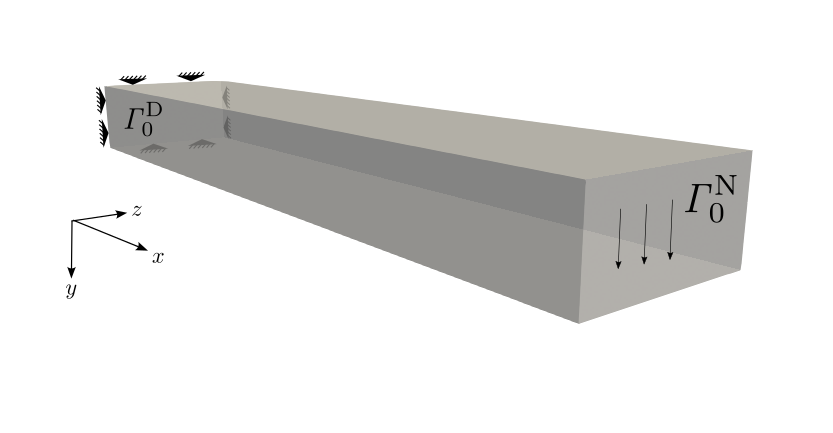
\includegraphics[width=0.85\textwidth]{fig/cantilever_setup.png}
\caption{Cantilever, problem setup.}
\label{fig:cantilever_setup}
\end{figure}

Study the setup shown in fig. \ref{fig:cantilever_setup} and the comments in the input file \verb"solid_cantilever.py" Run the simulation, either in one of the provided Docker containers or using your own FEniCSx/Ambit installation, using the command

\begin{verbatim}
mpiexec -n 1 python3 solid_cantilever.py
\end{verbatim}

It is fully sufficient to use one core (\verb"mpiexec -n 1") for the presented setup.

Open the results file \verb"results_solid_cantilever_displacement.xdmf" in Paraview, and visualize the deformation over time.

Figure \ref{fig:cantilever_results} shows the displacement magnitude at the end of the simulation.

\begin{figure}
\centering
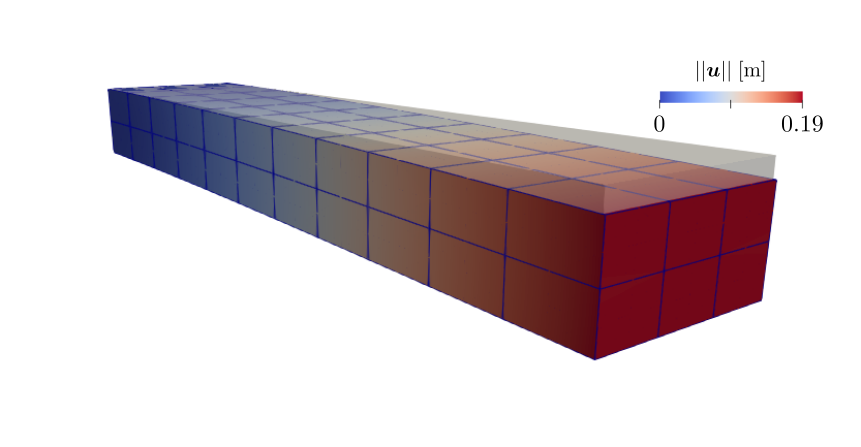
\includegraphics[width=0.85\textwidth]{fig/cantilever_results.png}
\caption{Cantilever, tip deformation. Color shows displacement magnitude.}
\label{fig:cantilever_results}
\end{figure}


\subsection{Demo: Fluid}\label{demo-fluid}

-- Physics description given in sec. \ref{fluid-mechanics}\\

-- Input files: \verb"demos/fluid"

\subsubsection*{2D channel flow}

This example shows how to set up 2D fluid flow in a channel around a rigid obstacle. Incompressible Navier-Stokes flow is solved using Taylor-Hood elements
(9-node biquadratic quadrilaterals for the velocity, 4-node bilinear quadrilaterals for the pressure).

\begin{figure}
\centering
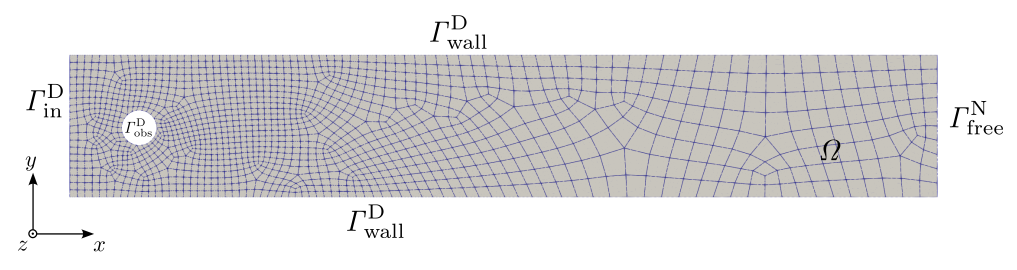
\includegraphics[width=0.9\textwidth]{fig/channel_setup.png}
\caption{Channel flow, problem setup.}
\label{fig:channel_setup}
\end{figure}

Study the setup and the comments in the input file \verb"fluid_channel.py". Run the simulation, either in one of the provided Docker containers or using your own FEniCSx/Ambit installation, using the command

\begin{verbatim}
mpiexec -n 1 python3 fluid_channel.py
\end{verbatim}

It is fully sufficient to use one core (\verb"mpiexec -n 1") for the presented setup.

Open the results file \verb"results_fluid_channel_velocity.xdmf" and \\ \verb"results_fluid_channel_pressure.xdmf" in Paraview, and visualize the velocity as well as the pressure over time.

Fig. \ref{fig:channel_results} shows the velocity magnitude (top) as well as the pressure (bottom part) at the end of the simulation.

\begin{figure}[ht]
\centering
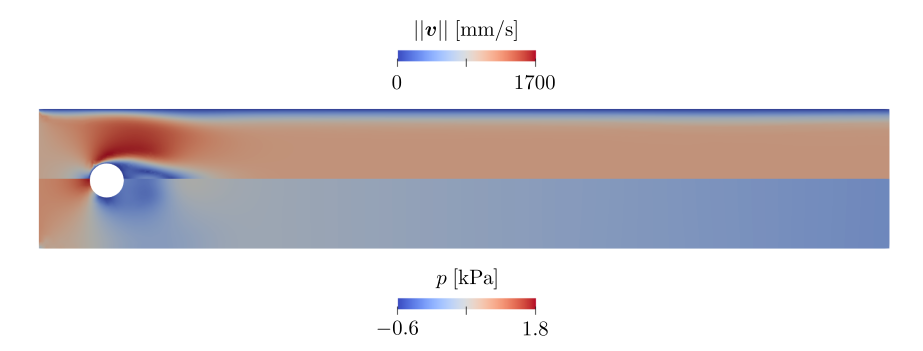
\includegraphics[width=0.9\textwidth]{fig/channel_results.png}
\caption{Velocity magnitude (top part) and pressure (bottom part) at end of simulation.}
\label{fig:channel_results}
\end{figure}


\subsection{Demo: 0D flow}\label{demo-0d-flow}

-- Physics description given in sec. \ref{d-flow-lumped-parameter-models}\\

-- Input files: \verb"demos/flow0d"

\subsubsection*{Systemic and pulmonary circulation}

This example demonstrates how to simulate a cardiac cycle using a lumped-parameter (0D) model for the heart chambers and the entire circulation. Multiple heart beats are run
until a periodic state criterion is met (which compares variable values at the beginning to those at the end of a cycle, and stops if the relative change is less than
a specified value, here \verb"`eps_periodic'" in the \verb"TIME_PARAMS" dictionary). The problem is set up such that periodicity is reached after 5 heart cycles.

\begin{figure}
\centering
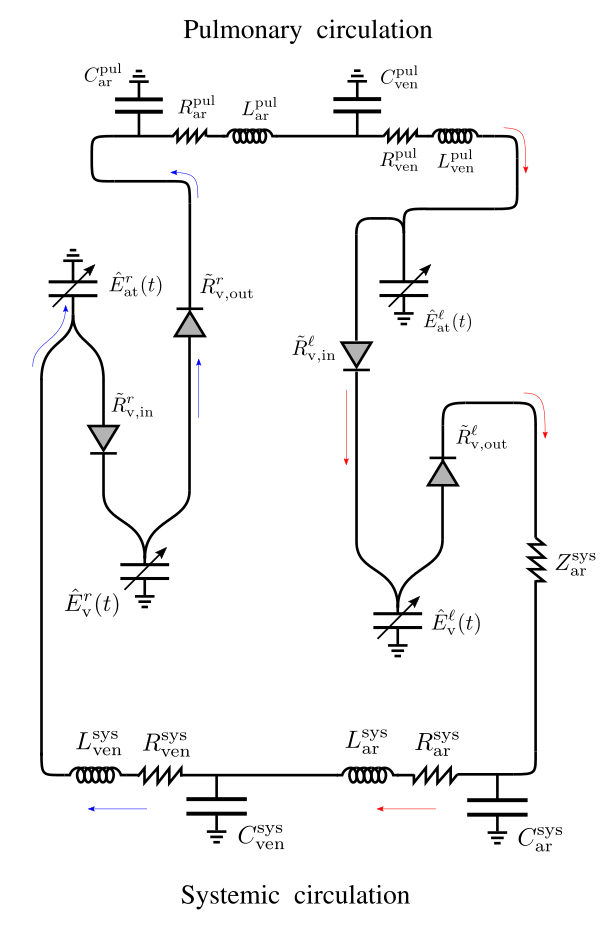
\includegraphics[width=0.65\textwidth]{fig/syspul_setup.png}
\caption{0D heart, systemic and pulmonary circulation, problem setup.}
\label{fig:syspul_setup}
\end{figure}

Study the setup in fig. \ref{fig:syspul_setup} and the comments in the input file \verb"flow0d_heart_cycle.py". Run the simulation, either in one of the provided Docker containers or using your own FEniCSx/Ambit installation, using the command
\begin{verbatim}
python3 flow0d_heart_cycle.py
\end{verbatim}

For postprocessing of the time courses of pressures, volumes, and fluxes of the 0D model, either use your own tools to plot the text output files (first column is time, second is the respective quantity), or make sure to have Gnuplot (and TeX) installed and navigate to the output folder (\verb"tmp/") in order to execute the script \verb"flow0d_plot.py" (which lies in \verb"ambit/src/ambit_fe/postprocess/"):
\begin{verbatim}
flow0d_plot.py -s flow0d_heart_cycle -n 100
\end{verbatim}
A folder \verb"plot_flow0d_heart_cycle" is created inside \verb"tmp/". Look at the results of pressures ($p$), volumes ($V$), and fluxes ($q$, $Q$) over time.
Subscripts \verb"v", \verb"at", \verb"ar", \verb"ven" refer to `ventricular', `atrial', `arterial', and `venous', respectively. Superscripts \verb"l", \verb"r", \verb"sys", \verb"pul" refer to `left', `right', `systemic', and
`pulmonary', respectively.
Try to understand the time courses of the respective pressures, as well as the plots of ventricular pressure over volume.
Check that the overall system volume is constant and around 4-5 liters.\\

The solution is depicted in fig. \ref{fig:syspul_results}, showing the time course of volumes and pressures of the circulatory system.

\begin{figure}
\centering
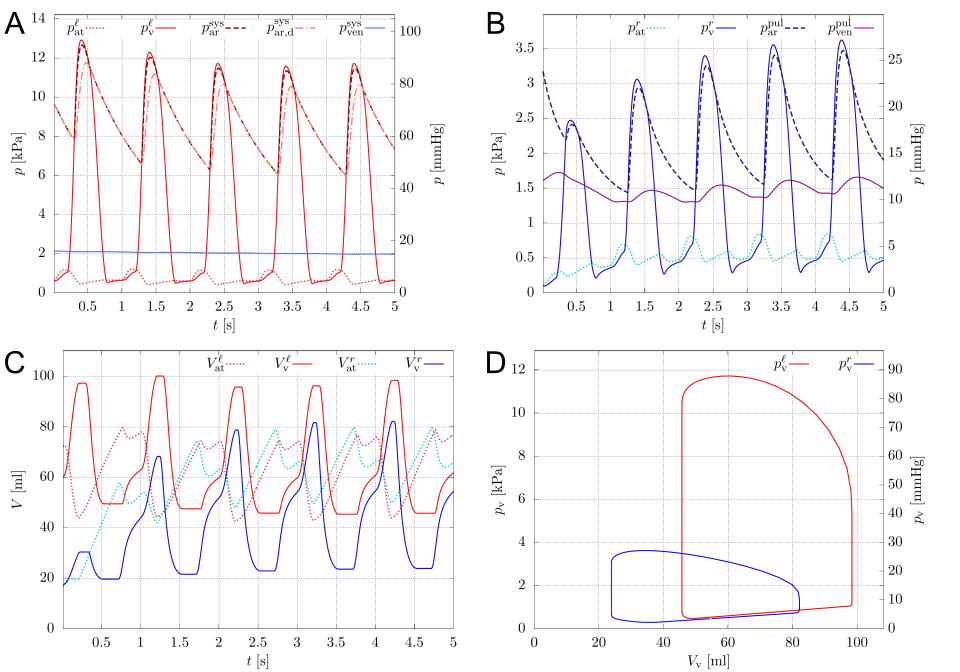
\includegraphics[width=1.0\textwidth]{fig/syspul_results.png}
\caption{A. Left heart and systemic pressures over time. B. Right heart and pulmonary pressures over time. C. Left and right ventricular and atrial volumes over time. D. Left and right ventricular pressure-volume relationships of periodic (5th) cycle.}
\label{fig:syspul_results}
\end{figure}


\subsection{Demo: Solid + 0D flow}\label{demo-solid-0d-flow}

-- Physics description given in sec. \ref{solid-0d-flow}\\

-- Input files: \verb"demos/solid_flow0d"

\subsubsection*{3D heart, coupled to systemic and pulmonary circulation}

This example demonstrates how to set up and simulate a two-chamber (left and right ventricular) solid mechanics heart model coupled to a closed-loop
0D circulatory system. A full dynamic heart cycle of duration 1 s is simulated, where the active contraction is modeled by a prescribed active stress approach.
Passive material behavior of the heart muscle is governed by the Holzapfel-Ogden anisotropic strain energy function \cite{holzapfel2009} and a strain rate-dependent viscous model \cite{chapelle2012}.
We start the simulation with "prestressing" using the MULF method \cite{gee2010,schein2021}, which allows to imprint loads without changing the geometry,
where the solid is loaded to the initial left and right ventricular pressures.
Thereafter, we kickstart the dynamic simulation with passive ventricular filling by the systole of the atria (0D chamber models). Ventricular systole
happens in $t \in [0.2\;\mathrm{s}, 0.53\;\mathrm{s}]$, hence lasting a third of the whole cycle time. After systole, the heart relaxes and eventually fills to about the same pressure
as it has been initialized to.\\

NOTE: For demonstrative purposes, a fairly coarse finite element discretization is chosen here, which by no means yields a spatially converged solution and which
may be prone to locking phenomena. The user may increse the parameter \verb"`order_disp'" in the \verb"FEM_PARAMS" section from \verb"1" to \verb"2" (and increase \verb"`quad_degree'" to \verb"6") such that quadratic finite element ansatz functions (instead of linear ones) are used. While this will increase accuracy and mitigate locking, computation time will
increase.

\begin{figure}
\centering
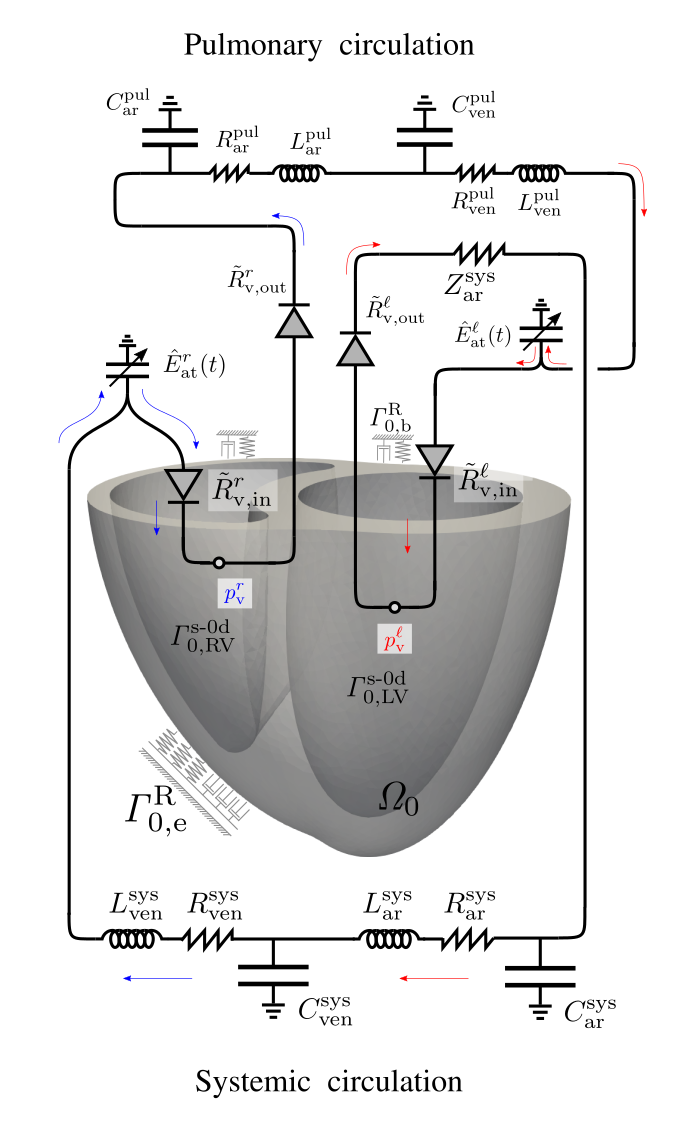
\includegraphics[width=0.65\textwidth]{fig/heart_syspul_setup.png}
\caption{Generic 3D ventricular heart model coupled to a closed-loop systemic and pulmonary circulation model.}
\label{fig:heart_syspul_setup}
\end{figure}

Study the setup shown in fig. \ref{fig:heart_syspul_setup} and the comments in the input file \verb"solid_flow0d_heart_cycle.py". Run the simulation, either in one of the provided Docker containers or using your own FEniCSx/Ambit installation, using the command
\begin{verbatim}
mpiexec -n 1 python3 solid_flow0d_heart_cycle.py
\end{verbatim}

It is fully sufficient to use one core (\verb"mpiexec -n 1") for the presented setup, while you might want to use more (e.g., \verb"mpiexec -n 4") if you increase \verb"`order_disp'" to \verb"2".

Open the results file \verb"results_solid_flow0d_heart_cycle_displacement.xdmf" in Paraview, and visualize the deformation over the heart cycle.

For postprocessing of the time courses of pressures, volumes, and fluxes of the 0D model, either use your own tools to plot the text output files (first column is time, second is the respective quantity), or make sure to have Gnuplot (and TeX) installed and navigate to the output folder (\verb"tmp/") in order to execute the script \verb"flow0d_plot.py" (which lies in \verb"ambit/src/ambit_fe/postprocess/"):
\begin{verbatim}
flow0d_plot.py -s solid_flow0d_heart_cycle -V0 117e3 93e3 0 0 0
\end{verbatim}

A folder \verb"plot_solid_flow0d_heart_cycle" is created inside \verb"tmp/". Look at the results of pressures ($p$), volumes ($V$), and fluxes ($q$, $Q$) over time.
Subscripts \verb"v", \verb"at", \verb"ar", \verb"ven" refer to `ventricular', `atrial', `arterial', and `venous', respectively. Superscripts \verb"l", \verb"r", \verb"sys", \verb"pul" refer to `left', `right', `systemic', and
`pulmonary', respectively.
Try to understand the time courses of the respective pressures, as well as the plots of ventricular pressure over volume.
Check that the overall system volume is constant and around 4-5 liters.\\

NOTE: This setup computes only one cardiac cycle, which does not yield a periodic state solution (compare e.g. initial and end-cyclic right ventricular pressures and volumes,
which do not coincide). Change the parameter \verb"number_of_cycles" from \verb"1" to \verb"10" and re-run the simulation. The simulation will stop when the cycle error (relative change in 0D variable quantities from beginning to end of a cycle) falls below the value of \verb"`eps_periodic'" (set to $5 \%$). How many cycles are needed to reach periodicity?\\

Figure \ref{fig:heart_syspul_results} shows a high-fidelity solution using a refined mesh and quadratic tetrahedral elements. Compare your solution from the coarser mesh. What is the deviation
in ventricular volume?

\begin{figure}
\centering
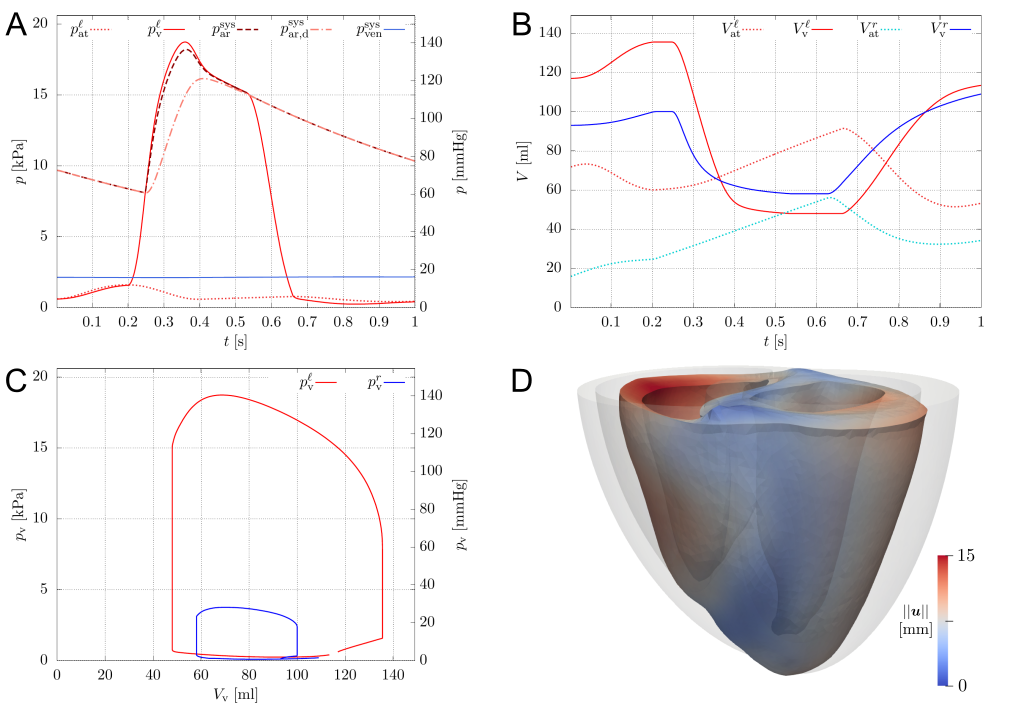
\includegraphics[width=1.0\textwidth]{fig/heart_syspul_results.png}
\caption{A. Left heart and systemic pressures over time. B. Left and right ventricular and atrial volumes over time. C. Left and right ventricular pressure-volume relationships. D. Snapshot of heart deformation at end-systole, color indicates displacement magnitude.}
\label{fig:heart_syspul_results}
\end{figure}


\subsection{Demo: Fluid + 0D flow}\label{demo-fluid-0d-flow}

-- Physics description given in sec. \ref{fluid-0d-flow}\\

-- Input files: \verb"demos/fluid_flow0d"

\subsubsection*{Blocked pipe flow with 0D model bypass}

\textit{\textbf{Note:} This demo only runs with the mixed dolfinx branch, which is pre-installed in the Ambit devenv Docker container. Pull this container and install Ambit in there according to the instructions in sec. \ref{installation}.}\\

This example demonstrates how to couple 3D fluid flow to a 0D lumped-parameter model. Incompressible transient Navier-Stokes flow in a pipe with prescribed inflow is solved,
with the special constraint that an internal boundary (all-time closed valve) separates region 1 and region 2 of the pipe. This internal Dirichlet condition can only be achieved
by splitting the pressure space, hence having duplicate pressure nodes at the valve plane. Otherwise, fluid would experience deceleration towards the valve and unphysical acceleration behind it, since the pressure gradient drives fluid flow. To achieve this, the mixed Dolfinx branch instead of the main branch is used. It is installed inside the Ambit devenv Docker
container. In the future, this functionality is expected to be merged into the Dolfinx main branch (at least it was announced...).\\

This example demonstrates how the closed valve can be bypassed by a 0D flow model that links the 3D fluid out-flow of one region to the in-flow of the other region. The 0D model consists of two Windkessel models in series, each having compliance, resistance, and inertance elements.

\begin{figure}
\centering
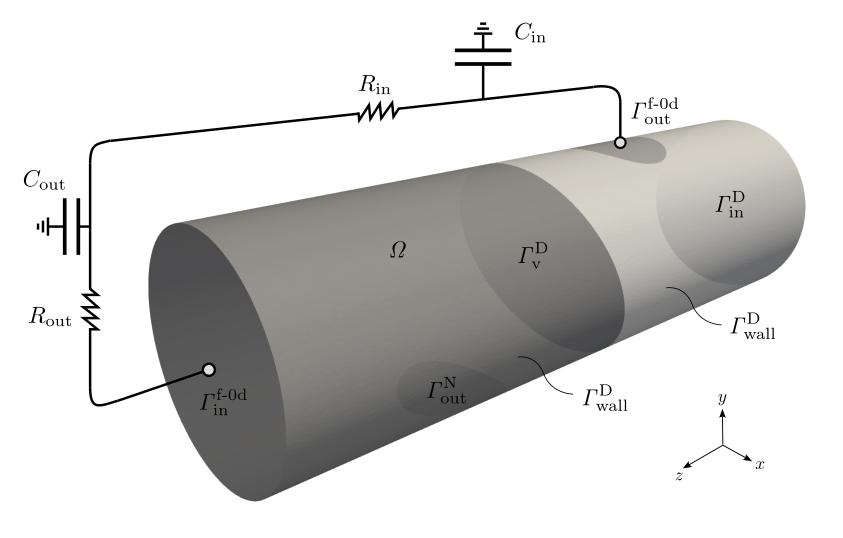
\includegraphics[width=0.85\textwidth]{fig/pipe_0d_setup.png}
\caption{Blocked pipe with 0D model bypass, simulation setup.}
\label{fig:pipe_0d_setup}
\end{figure}

Study the setup shown in fig. \ref{fig:pipe_0d_setup} and the comments in the input file \verb"fluid_flow0d_pipe.py". Run the simulation, either in one of the provided Docker containers or using your own FEniCSx/Ambit installation, using the command
\begin{verbatim}
mpiexec -n 1 python3 fluid_flow0d_pipe.py
\end{verbatim}
It is fully sufficient to use one core (\verb"mpiexec -n 1") for the presented setup.

Open the results file \verb"results_fluid_flow0d_pipe_velocity.xdmf" in Paraview, and visualize the velocity over time.

Think of which parameter(s) of the 0D model to tweak in order to achieve a) little to no fluid in-flow (into $\mathit{\Gamma}_{\mathrm{in}}^{\mathrm{f\text{-}0d}}$), b) almost the same flow across $\mathit{\Gamma}_{\mathrm{out}}^{\mathrm{f\text{-}0d}}$ and $\mathit{\Gamma}_{\mathrm{in}}^{\mathrm{f\text{-}0d}}$. Think of where the flow is going to in case of a).\\

Figure shows the velocity streamlines and magnitude at the end of the simulation.

\begin{figure}
\centering
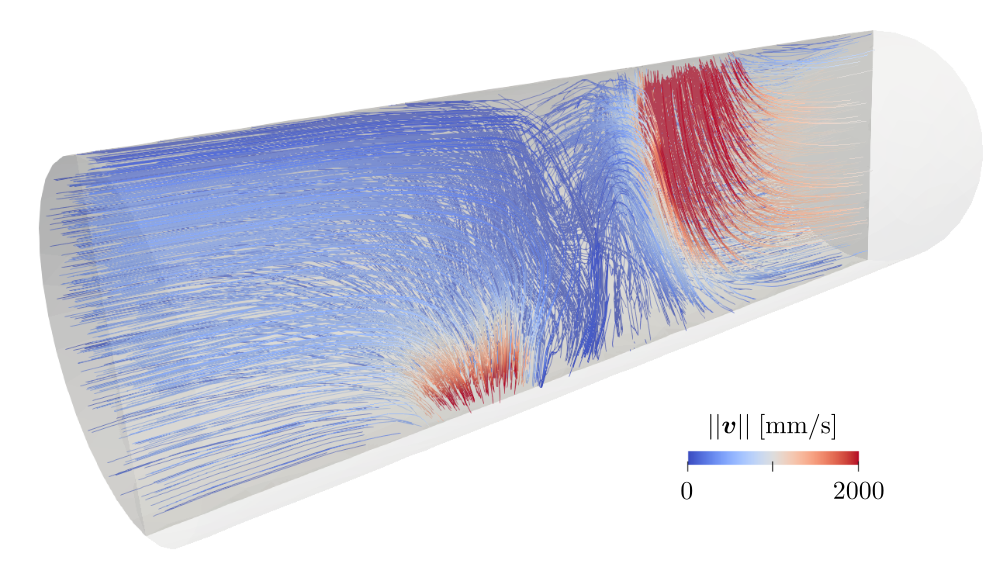
\includegraphics[width=0.85\textwidth]{fig/pipe_0d_results.png}
\caption{Streamlines of velocity at end of simulation, color indicates velcity magnitude.}
\label{fig:pipe_0d_results}
\end{figure}


\subsection{Demo: FSI}\label{demo-fsi}

-- Physics description given in sec. \ref{fluid-solid-interaction-fsi}\\

-- Input files: \verb"demos/fsi"\\

\textit{\textbf{Note:} FSI only runs with the mixed dolfinx branch, which is pre-installed in the Ambit devenv Docker container. Pull this container and install Ambit in there according to the instructions in sec. \ref{installation}.}

\subsubsection*{Channel flow around elastic flag}

Incompressible fluid flow in a 2D channel around an elastic flag is studied. The setup corresponds to the well-known Turek benchmark \cite{turek2006}. Here, the two cases FSI2 and FSI3 from the original setup are investigated. A prescribed inflow velocity with parabolic inflow profile is used:\\
\begin{equation}
\begin{aligned}
    \vf = \bar{v}(t,y) \bs{e}_{x}
    \quad &  
    \text{on}\; \Gm_{t,\mathrm{in}}^{D,\fF} \times [0,T],
    \label{eq:flag_dbc_in}
\end{aligned}
\end{equation}
with 
\begin{equation}
\begin{aligned}
    \bar{v}(t,y) = \begin{cases} 1.5 \,\bar{U}\, \frac{y(H-y)}{\left(\frac{H}{2}\right)^2} \frac{1-\cos\left(\frac{\pi}{2}t\right)}{2}, & \text{if} \; t < 2, \\ 1.5 \,\bar{U}\, \frac{y(H-y)}{\left(\frac{H}{2}\right)^2}, & \text{else}, \end{cases}
    \label{eq:flag_dbcs_func}
\end{aligned}
\end{equation}

with $\bar{U}=10^{3}\;\mathrm{mm}/\mathrm{s}$ (FSI2) and $\bar{U}=2\cdot 10^{3}\;\mathrm{mm}/\mathrm{s}$ (FSI3).\\

\begin{figure}
\centering
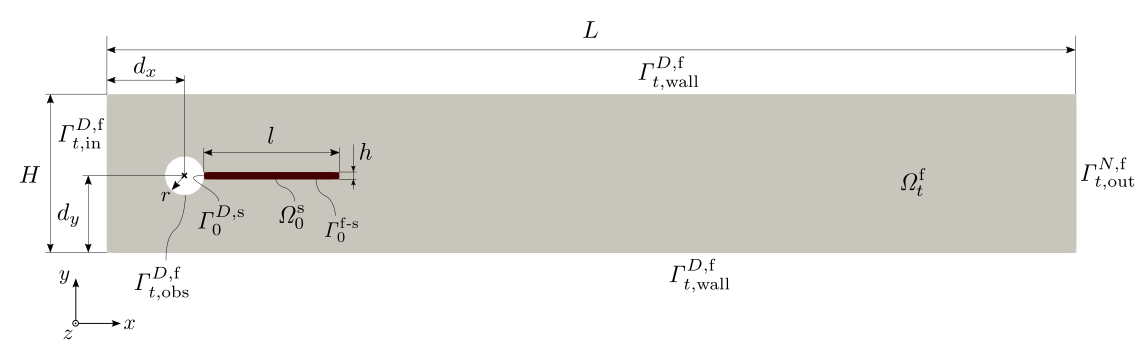
\includegraphics[width=1.0\textwidth]{fig/channel_flag_setup.png}
\caption{Channel flow around an elastic flag \cite{turek2006}, problem setup.}
\label{fig:channel_flag_setup}
\end{figure}

Geometrical parameters, given in $[\mathrm{mm}]$, are:
\begin{table}[!h]
\begin{center}
%\caption{Geometrical parameters of modified Turek's benchmark, in $[\mathrm{mm}]$}\label{tab:params_geo_turek}
\begin{tabular}{ccccccc}
 $L$    & $H$   & $r$  & $l$   & $h$  & $d_x$ & $d_y$ \\\hline
 2500 & 410 & 50 & 350 & 20 & 200 & 200 
\end{tabular}
\end{center}
\end{table}

Both solid and fluid are discretized with quadrilateral $\mathbb{Q}^2$-$\mathbb{Q}^1$ Taylor-Hood finite elements, hence no stabilization for the fluid problem is needed. Temporal discretization for both the solid and the fluid are carried out with a Generalized-$\alpha$ scheme with no numerical damping ($\rho_{\mathrm{inf}}=1$).\\

Study the setup shown in fig. \ref{fig:channel_flag_setup} together with the parameters in the table and the comments in the input file \verb"fsi_channel_flag.py". Run the simulation for FSI2 and FSI3 cases, either in one of the provided Docker containers or using your own FEniCSx/Ambit installation, using the command
\begin{verbatim}
mpiexec -n 1 python3 fsi_channel_flag.py
\end{verbatim}

If your system allows, use more than one core (e.g. \verb"mpiexec -n 4") in order to speed up the simulation a bit.\\

The physics of the problem are strongly time-dependent, and a (near-)periodic oscillation of the flag only occurs after $t\approx 10\;\mathrm{s}$ (FSI2) and $t\approx 5\;\mathrm{s}$ (FSI3). Run the problem to the end ($t = 15\;\mathrm{s}$ for FSI2, $t = 7.5\;\mathrm{s}$ for FSI3), be patient, and monitor the flag tip displacement over time.\\

Figure \ref{fig:channel_flag_results} depicts the velocity at three instances in time towards the end of the simulation for the FSI2 case, and figure \ref{fig:channel_flag_results_verif} shows the flag's tip displacement over time compared to the reference solution, over a time interval where the solution has become periodic. (Note that the reference solution from the official link shown in the input file needs to be time-adjusted, i.e. synchronized with the first peak in the interval of interest, since the time column of the reference data does not correspond to the physical time of the problem setup.)

\begin{figure}
\centering
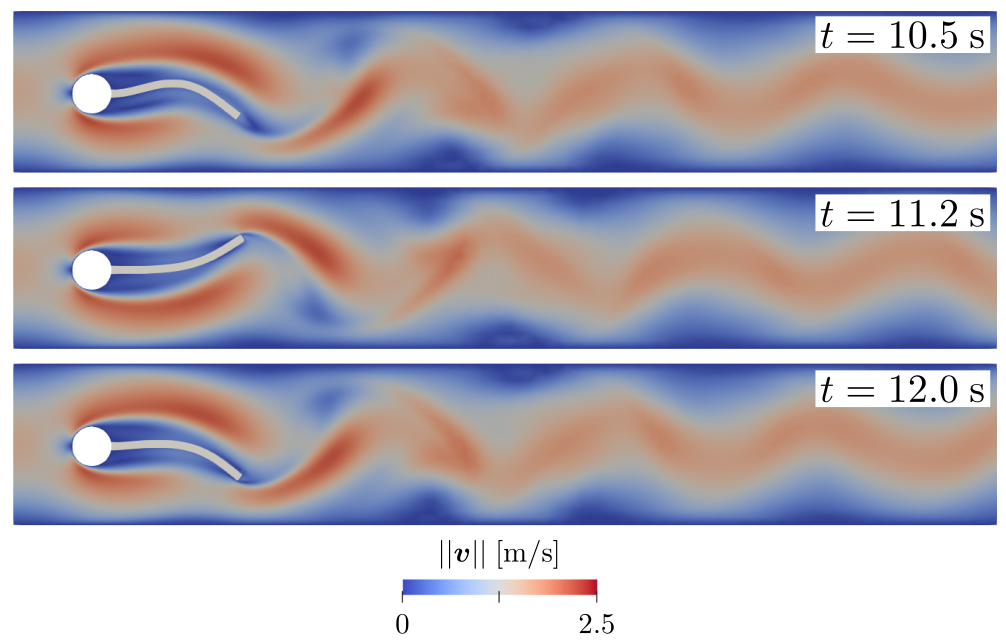
\includegraphics[width=0.85\textwidth]{fig/channel_flag_results.png}
\caption{FSI2 case: Magnitude of fluid velocity at three instances in time ($t=10.5\;\mathrm{s}$, $t=11.2\;\mathrm{s}$, and $t=12\;\mathrm{s}$) towards end of simulation, color indicates velcity magnitude.}
\label{fig:channel_flag_results}
\end{figure}


\begin{figure}
\centering
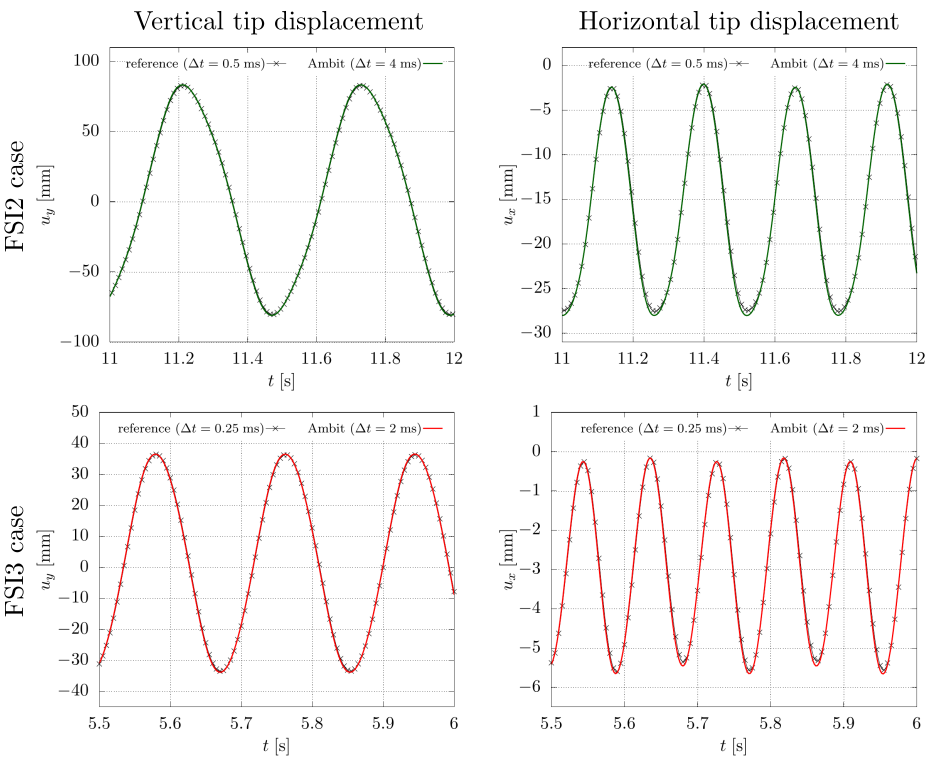
\includegraphics[width=1.0\textwidth]{fig/channel_flag_results_verif.png}
\caption{Comparison to benchmark reference solution for the time course of the flag's tip displacement for the two setups FSI2 and FSI3. A fairly coarse time step of $\Delta t = 4 \;\mathrm{ms}$ (FSI2) and $\Delta t = 2 \;\mathrm{ms}$ (FSI3) already allows a close match to the original results.}
\label{fig:channel_flag_results_verif}
\end{figure}


\clearpage

\section{Table of symbols}
\begin{equation}
\nonumber
\begin{aligned}
&\Om_0,\Om &&: \text{reference, current domain} \\
&\Gm_0,\Gm &&: \text{reference, current boundary} \\
&\bs{x}_0, \bs{x} &&: \text{coordinates of the reference, current frame} \\
&\bs{e}_x, \bs{e}_y, \bs{e}_z &&: \text{unit vectors of the cartesian reference frame} \\
&\bs{n}_0, \bs{n} &&: \text{unit outward normal defined in the reference, current frame} \\
&\bs{\nabla}_{0},\bs{\nabla} &&: \text{Nabla operator with respect to the reference, current frame} \\
&t, T &&: \text{current, end time of an initial boundary value problem} \\
&\bs{u}, \hat{\bs{u}}_{0} &&: \text{solid mechanics displacement field, and prescribed initial value} \\
&\delta\bs{u}, \Delta\bs{u} &&: \text{solid mechanics displacement test, trial function} \\
& p &&: \text{solid mechanics hydrostatic pressure, or fluid mechanics pressure} \\
& \delta p, \Delta p &&: \text{solid or fluid mechanics pressure test, trial function} \\
&\bs{v}=\frac{\mathrm{d}\bs{u}}{\mathrm{d}t}, \hat{\bs{v}}_{0} &&: \text{solid mechanics velocity, and prescribed initial value} \\
&\bs{a}=\frac{\mathrm{d}^2\bs{u}}{\mathrm{d}t^2} &&: \text{solid mechanics acceleration} \\
&\bs{v}, \hat{\bs{v}}_{0} &&: \text{fluid mechanics velocity, and prescribed initial value} \\
&\delta\bs{v}, \Delta\bs{v} &&: \text{fluid mechanics velocity test, trial function} \\
&\bs{a}=\frac{\partial\bs{v}}{\partial t} &&: \text{fluid mechanics acceleration} \\
&\bs{d}, \hat{\bs{d}}_{0} &&: \text{ALE displacement field, and prescribed initial value} \\
&\delta\bs{d}, \Delta\bs{d} &&: \text{ALE displacement test, trial function} \\
&\hat{\bs{b}}_0, \hat{\bs{b}} &&: \text{body force vector defined in the reference, current frame} \\
&\bs{w}=\frac{\mathrm{d}\bs{d}}{\mathrm{d}t}, \hat{\bs{w}}_{0} &&: \text{ALE velocity, and prescribed initial value} \\
&\rho_0, \rho &&: \text{reference, current density} \\
&\bs{P}=\bs{F}\bs{S} &&: \text{1st Piola Kirchhoff stress tensor} \\
&\bs{F}=\bs{I}+\bs{\nabla}_{0}\bs{u} &&: \text{solid deformation gradient} \\
&\widetilde{\bs{F}}=\bs{I}+\bs{\nabla}_{0}\bs{d} &&: \text{ALE deformation gradient} \\
&J=\det \bs{F} &&: \text{determinant of solid deformation gradient} \\
&\widetilde{J}=\det \widetilde{\bs{F}} &&: \text{determinant of ALE deformation gradient} \\
&\bs{S} &&: \text{2nd Piola-Kirchhoff stress tensor} \\
&\bs{\sigma} &&: \text{Cauchy stress tensor} \\
&\bs{t}_0, \hat{\bs{t}}_{0} &&: \text{1st Piola-Kirchhoff traction, prescribed 1st Piola-Kirchhoff traction} \\
&\bs{t}, \hat{\bs{t}} &&: \text{Cauchy traction, prescribed Cauchy traction} \\
\end{aligned}
\end{equation}

\newpage
\bibliography{ref}

\end{document}
